\documentclass[../main.tex]{subfiles}

\begin{document}
\providecommand{\localhost}{\lstinline{Macbook.local (192.168.2.15)}}
\providecommand{\server}{\lstinline{parrot.ece.mcgill.ca (132.206.75.13)}}
\section*{L4N1 Part 3}\addcontentsline{toc}{section}{L4N1 Part 3} 
\subsubsection*{List of Packets}
We filter the relevant packets to focus on the communication between the author's computer \localhost, and the server \server.\\
    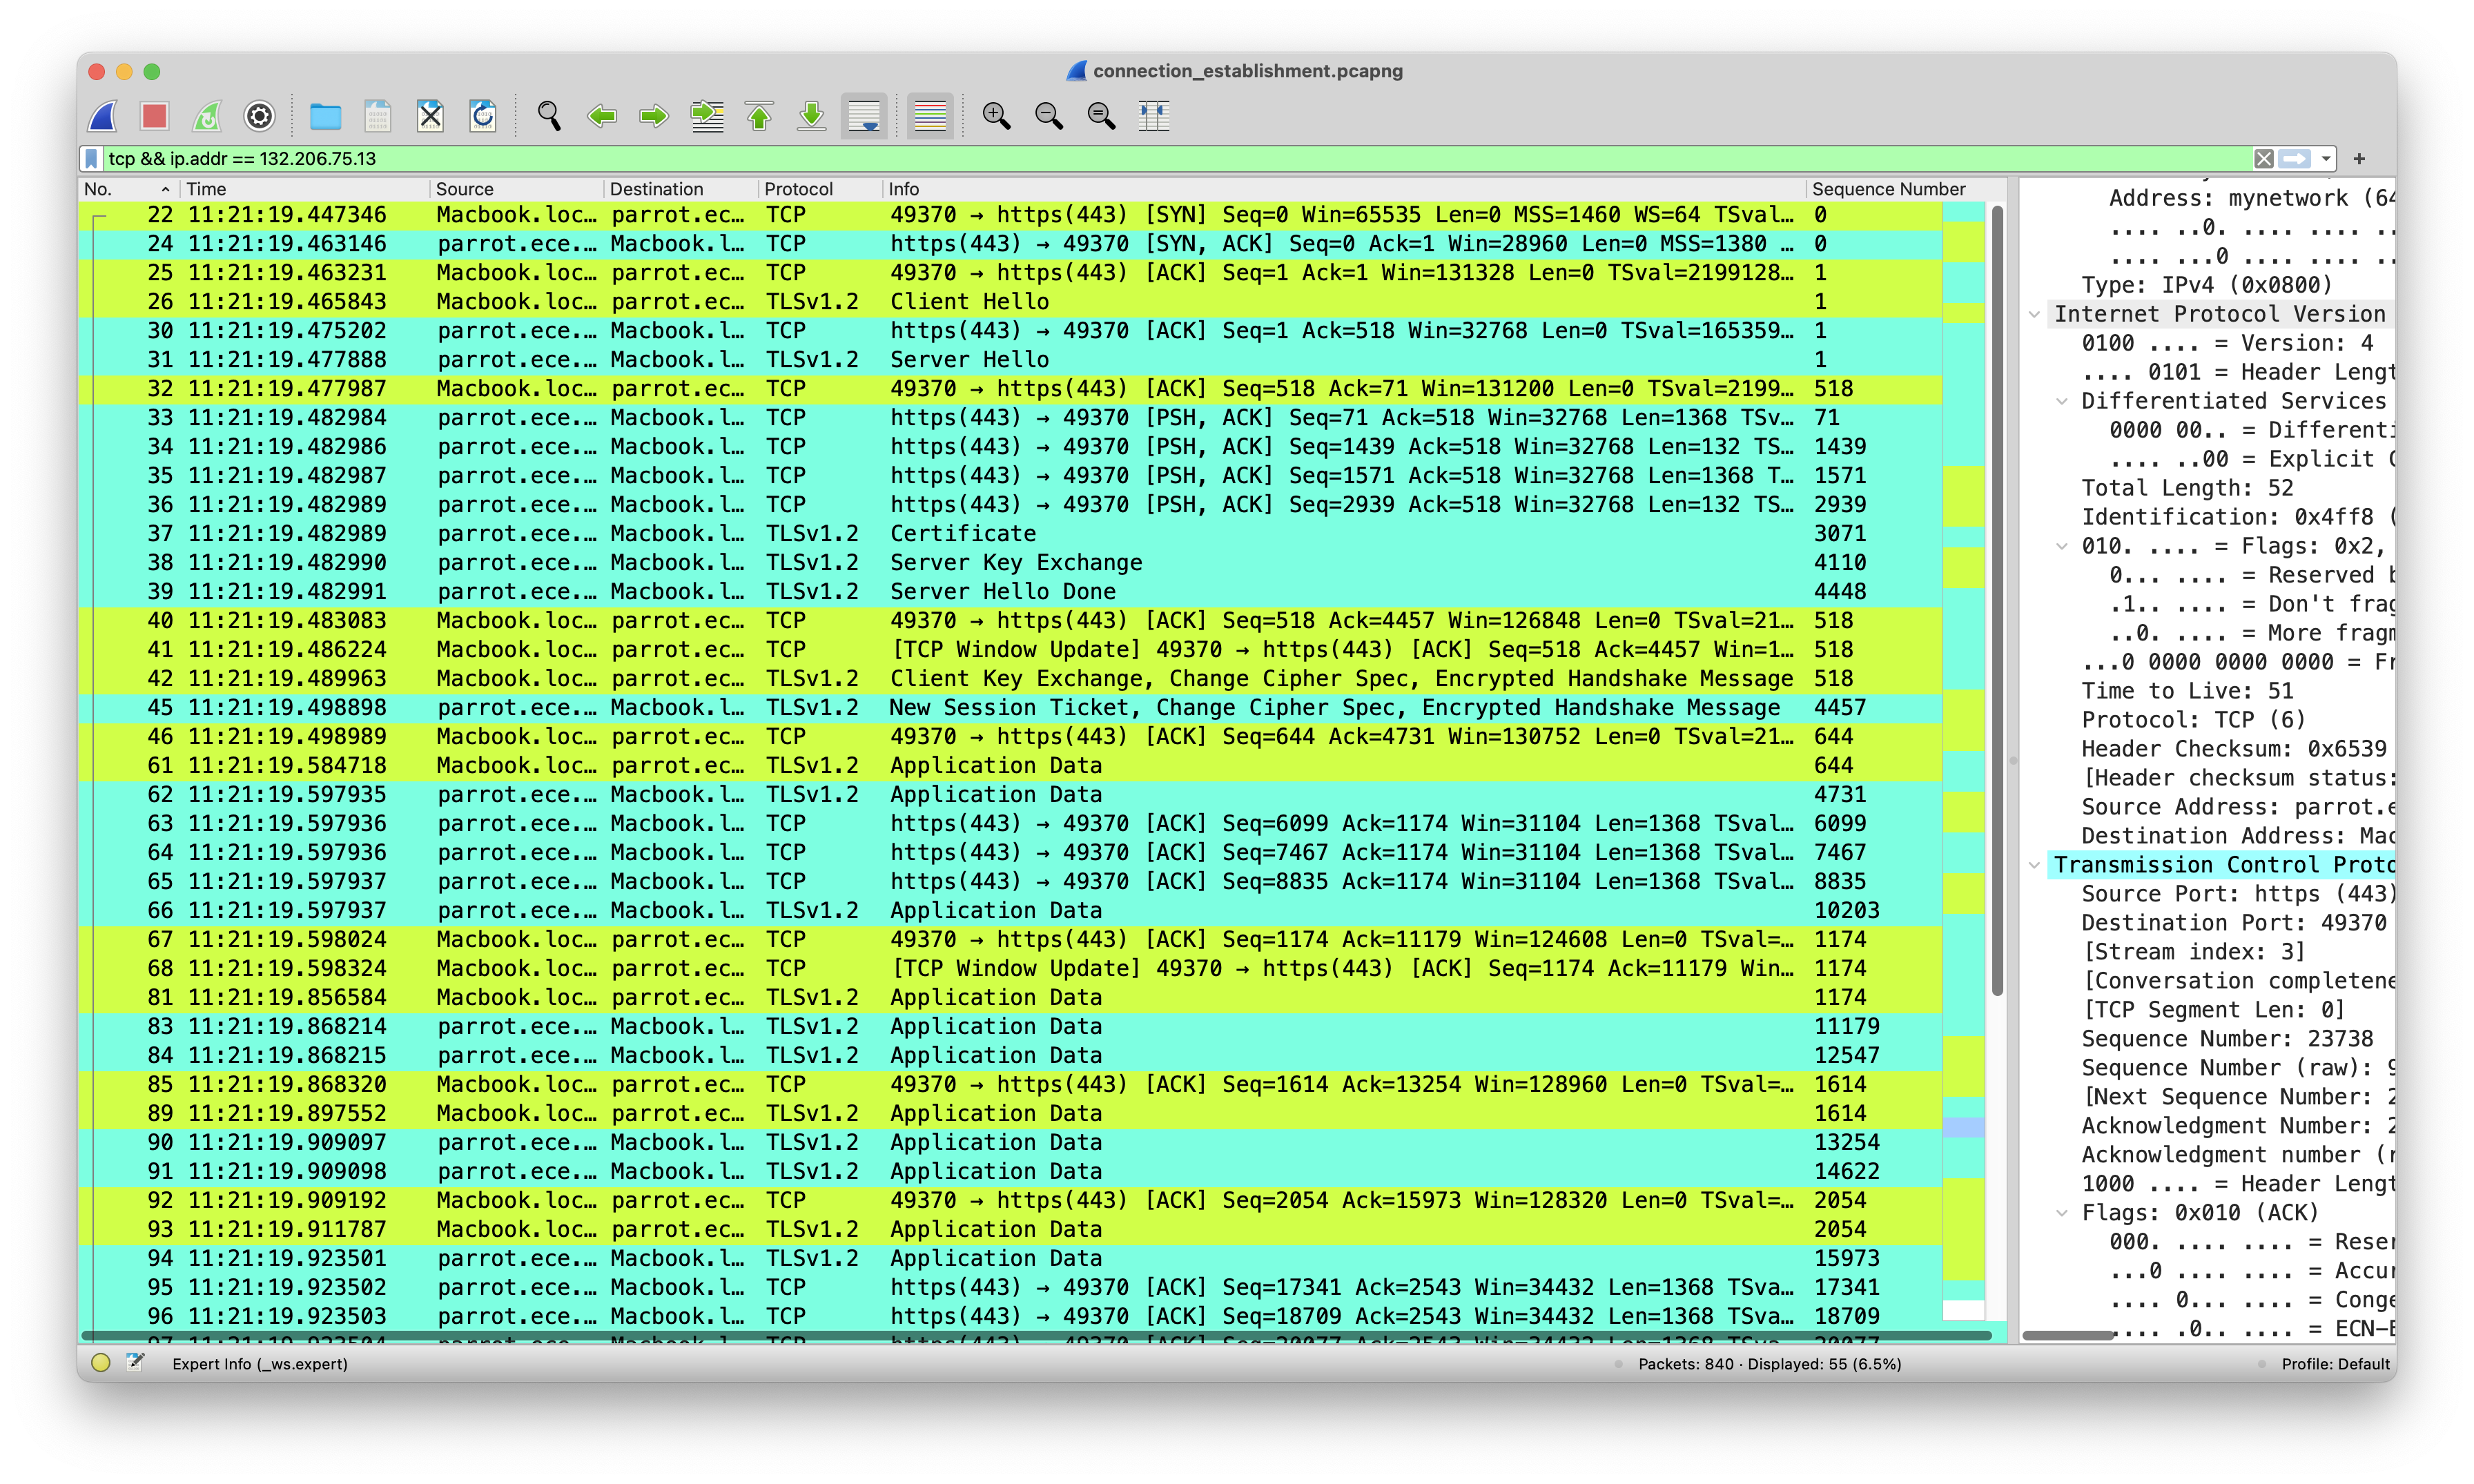
\includegraphics[width=\textwidth]{subfiles/images/L4N1_PAGE15_LIST_OF_PACKETS_1.png}
    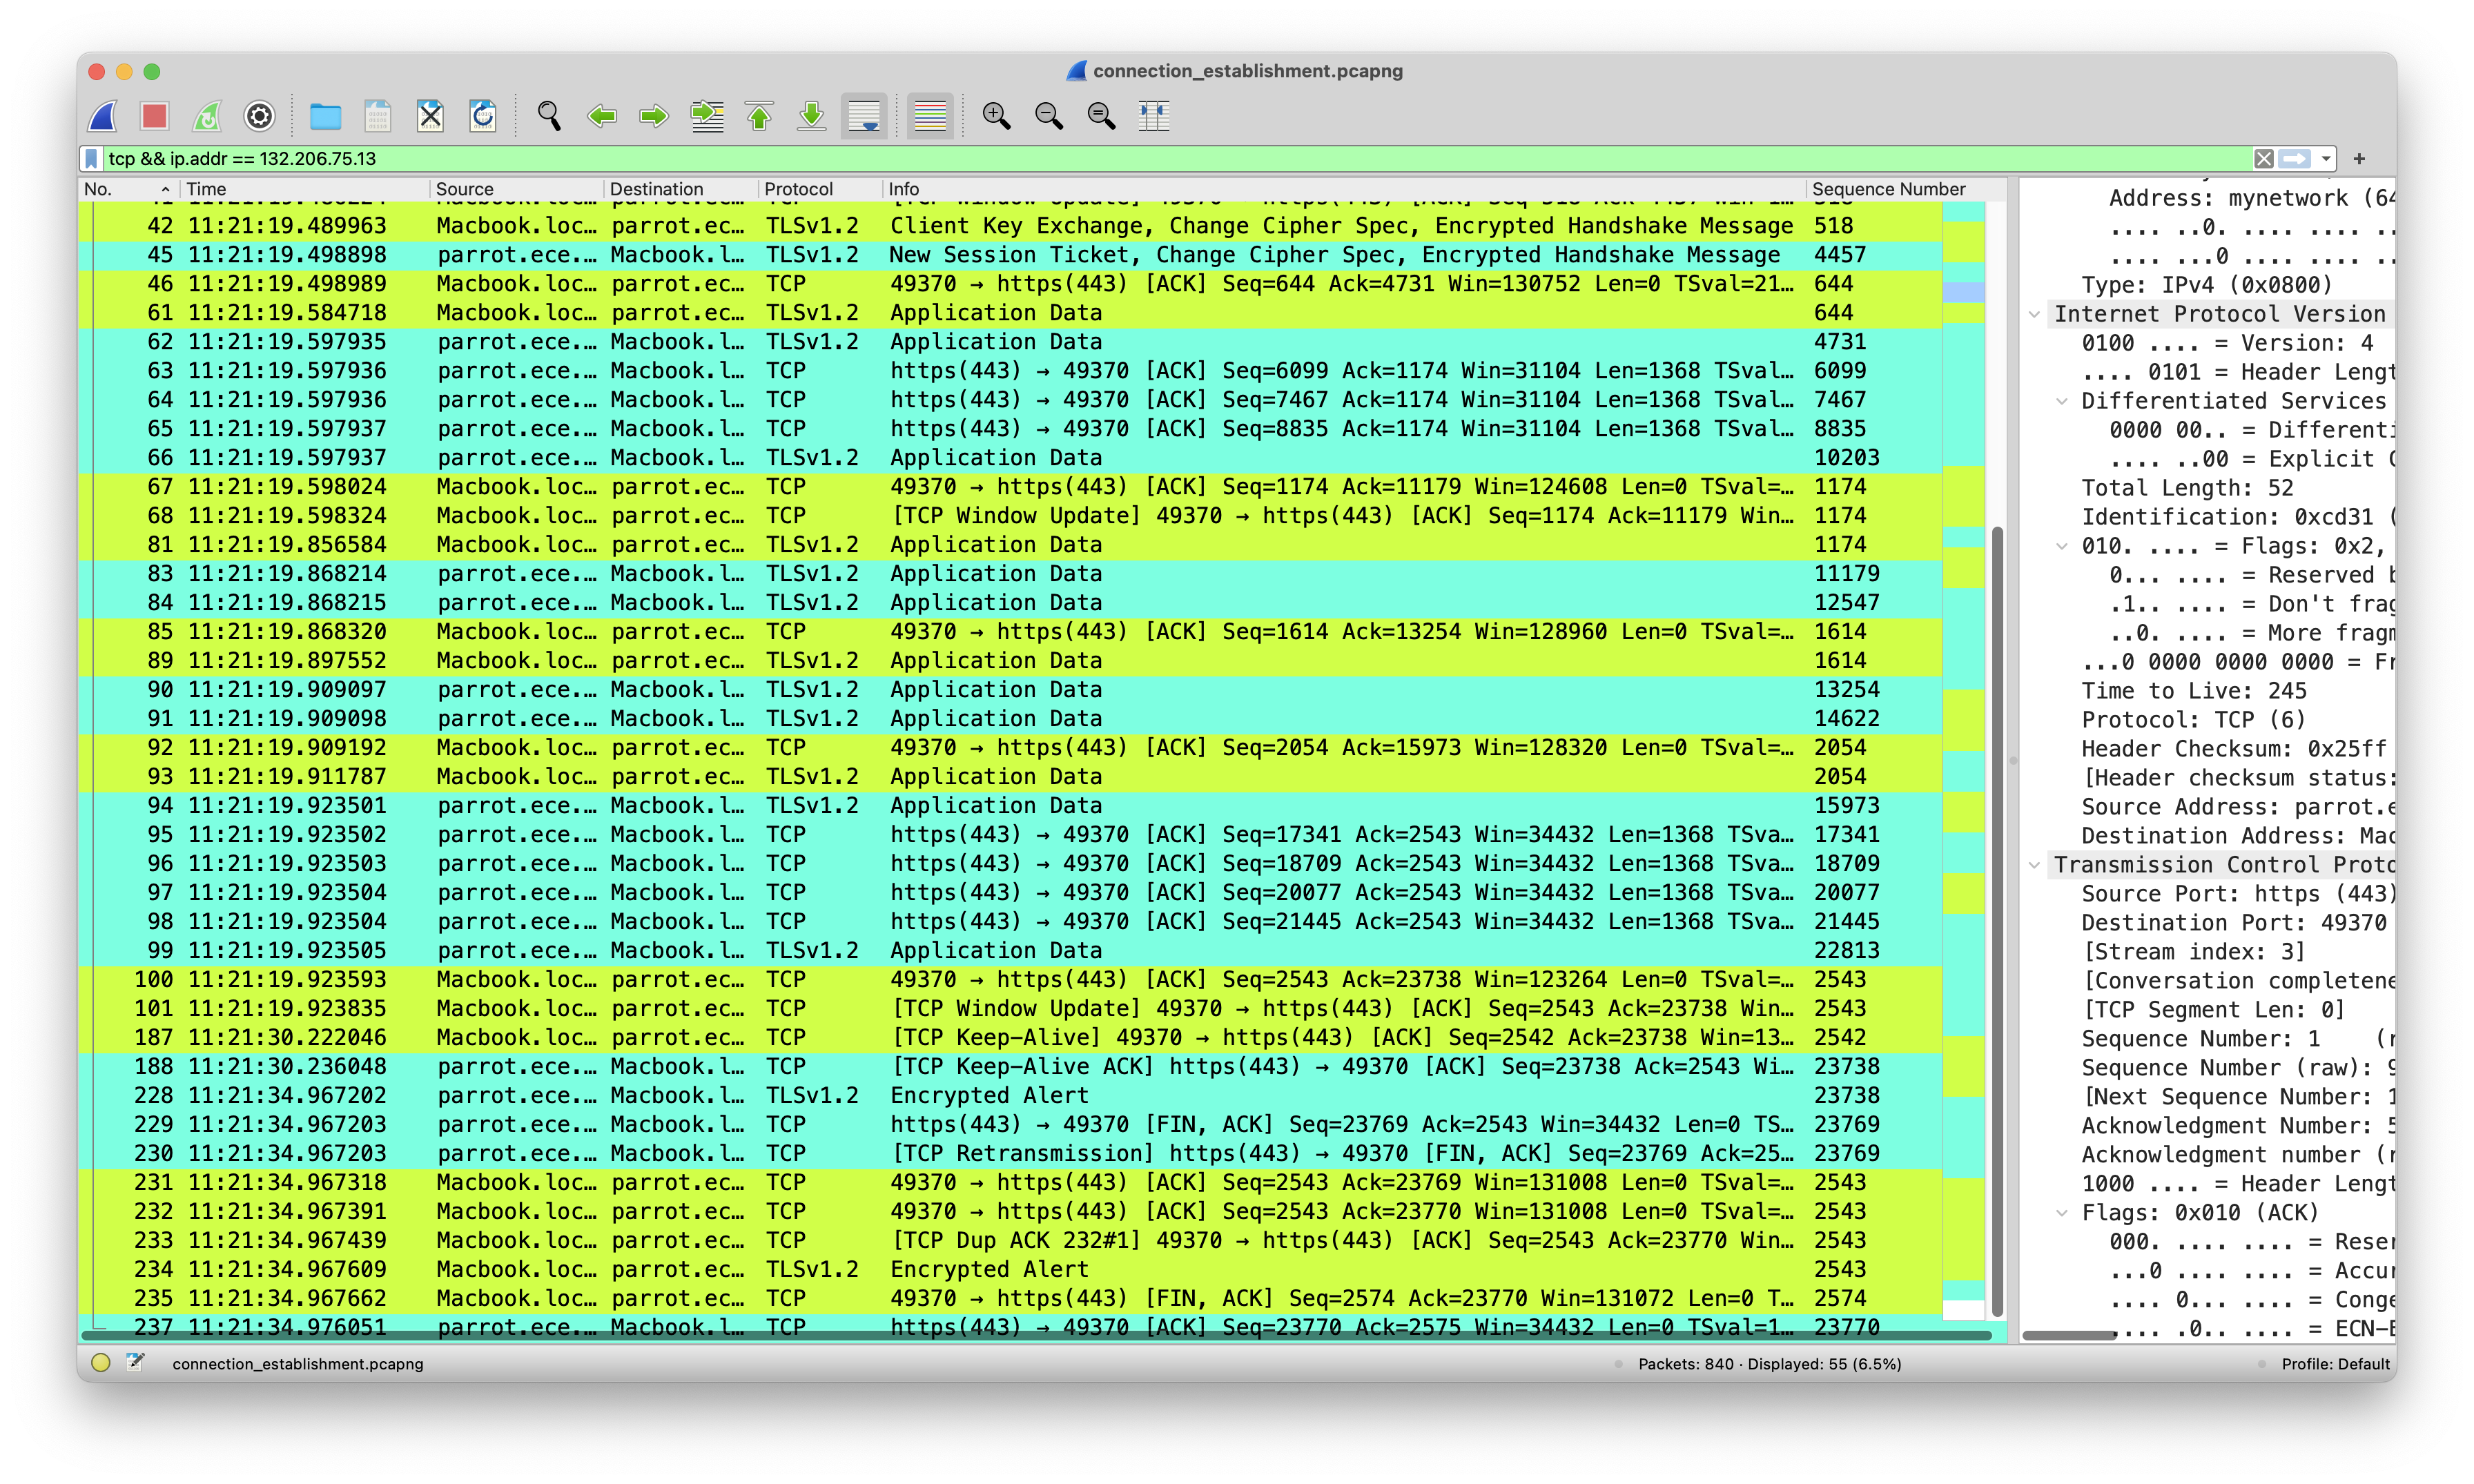
\includegraphics[width=\textwidth]{subfiles/images/L4N1_PAGE15_LIST_OF_PACKETS_2.png}
\newpage

\problem{1}
\begin{wts}
	How many TCP datagrams are exchanged between your computer and the server to establish the TCP connection? Why each of these segments is needed to setup the TCP connection?
\end{wts}
\begin{proof}
% Answer here
    There are three IP datagrams. Each of which contains a TCP segment. We will hereinafter discuss the three-way handshake process of TCP connection establishment.

\begin{quote}
    TCP is provides full-duplex data transport to the application layer by employing a sliding window mechanism. This requires both the sender and the receiver to maintain 1) the window size and 2) the expected sequence number of the other host, which advances (modulo $N$, where $N$ denotes the maximum sequence number) on the receipt of an acknowledgement.
\end{quote}
The first segment is sent from the client (the author’s computer) to the server, with the flag \code{SYN = 1}, and the client communicates to the server its
\begin{itemize}
    \item Window size $W_c$, the maximum number of bytes that the server should send without receiving an acknowledgement.
    \item Client initial sequence number, ${SEQ}_C$, a $32$-bit number 
\end{itemize}
Client wants the server to mind its window size in order to not overflow and cause packet loss. 
And for the server to configure its left window edge so that it is ready for the next Segment from the client. The client awaits the \code{ACK = x + 1} (modulo $N$), where
\begin{equation}\label{mod n}
N = \sup\biggl\{\norm{x},\,x\in\mathbb{B}^{32}\biggr\}\end{equation}

The server sends the second segment, with flags \code{SYN = 1}, and \code{ACK = x+1}, \code{SEQ = y}, and widow size $W_S$,
\begin{enumerate}
    \item Window size $W_s$, the maximum number of bytes the client should send without receiving an ACK from the server
    \item $SEQ_S$: Initial sequence number, a 32-bit number.
\end{enumerate} 
We note in passing that the maximum window size determined by any sliding window protocol, $w$, must also satisfy \[w< N2^{-1}\]When the client receives this \code{SYN-ACK}, it takes note of the server’s window size and adjusts the left window edge of its Transmit Control Buffer to \code{SEQ(server) + 1}, and sends an \code{ACK} back to the server.

In this third and last TCP segment, the client tells the server that it has configured its left window edge to \code{y+1} in its TCB, to be the same as the server’s RCB.

\end{proof}
\newpage

\problem{2}
\begin{wts}
	Which end point started the TCP Connection-Establishment phase?
\end{wts}
\begin{proof}
% Answer here
    The Firefox Web Browser Computer Digital Application on the author's computer \code{Macbook.local (192.168.2.15)} initiated the TCP connection establishment. 
\end{proof}
\newpage

\problem{3}
\begin{wts}
	What flags are set in each of these TCP datagrams?
\end{wts}
\begin{proof}
% Answer here
    We assume the question refers to a TCP segment, rather than an IP datagram. Consider the TCP Segments No. 22, 24, 25:\\
    \begin{itemize}
        \item Segment 22: Client to Server, Flags: \code{SYN}
        \begin{lstlisting}
        c0 da 01 bb 01 a3 ab af 00 00 00 00 b0 02 ff ff
        a6 2b 00 00 02 04 05 b4 01 03 03 06 01 01 08 0a
        83 14 0b 41 00 00 00 00 04 02 00 00\end{lstlisting}
        
        \item Segment 24: Server to Client, Flags: \code{SYN, ACK}
        \begin{lstlisting}
        01 bb c0 da 37 71 a3 41 01 a3 ab b0 a0 12 71 20
        20 85 00 00 02 04 05 64 04 02 08 0a 62 8f e8 86
        83 14 0b 41 01 03 03 07\end{lstlisting}
        
        \item Segment 25: Client to Server, Flags: \code{ACK}
         \begin{lstlisting}
        c0 da 01 bb 01 a3 ab b0 37 71 a3 42 80 10 08 04
        b8 0c 00 00 01 01 08 0a 83 14 0b 52 62 8f e8 86\end{lstlisting}
    \end{itemize}
    
    % \lstinputlisting{./L4N1_PAGE15_CONNECTION_ESTABLISH_PACKET_1.txt}
    % \lstinputlisting{./L4N1_PAGE15_CONNECTION_ESTABLISH_PACKET_2.txt}
    % \lstinputlisting{./L4N1_PAGE15_CONNECTION_ESTABLISH_PACKET_3.txt}
\end{proof}
\newpage

\problem{4}
\begin{wts}
	What is the initial value of the sequence number on the client’s side?
\end{wts}
\begin{proof}
% Answer here
    Initial Sequence Number (Client): 		\code{0x01a3abaf}
\end{proof}
\newpage

\problem{5}
\begin{wts}
	What is the initial value of the sequence number on the server’s side?
\end{wts}
\begin{proof}
% Answer here
    Initial Sequence Number (Server): 		\code{0x3771a341}
\end{proof}
\newpage

\problem{6}
\begin{wts}
	What is the value of the Acknowledgement field in the SYN ACK datagram? How did the server determine that value?
\end{wts}
\begin{proof}
% Answer here
    ACK value within SYN-ACK Segment: 	\code{0x01a3abb0}. The determination is from adding $1$ modulo $N$, (see Equation \eqref{mod n})
\end{proof}
\newpage


\problem{7}
\begin{wts}
	For the TCP SYN datagram, determine the following
	\begin{enumalpha}
		\item the source port number
		\item the destination port number
		\item the size of the window
		\item the header length
	\end{enumalpha}
\end{wts}
\begin{proof}
% Answer here
    TCP SYN datagram, determine
    \begin{enumalpha}
        \item source port 49370, 
        \item dest port 443,
        \item window size 65535 bytes,
        \item TCP segment header length 44 bytes.    
    \end{enumalpha}
\end{proof}
\newpage


\problem{8}
\begin{wts}
	For the TCP SYN ACK datagram, determine the following
	\begin{enumalpha}
		\item the source port number
		\item the destination port number
		\item the size of the window
		\item the header length
	\end{enumalpha}
\end{wts}
\begin{proof}
% Answer here
TCP SYN-ACK datagram, determine
\begin{enumalpha}
    \item source port 443 
	\item dest port 49370,
	\item window size 28960 bytes,
	\item TCP segment header length 40 bytes.
\end{enumalpha}
\end{proof}
\newpage


\problem{9}
\begin{wts}
	What is the usage of the window field in the TCP segments?
\end{wts}
\begin{proof}
% Answer here
    On an abstract level, an application process that resides on the host’s computer dedicates a buffer region in a transmit control block (TCB). The size the TCB is finite, so the sender must be aware of the remaining available buffer space left in the TCB. For the simple case where the application process reads the data immediately, in technical terms we say that the right window edge advances with the left — the ‘window’ field advertises the difference between the last byte sent and the last byte ACKed by the destination TCP.\\

    If we relax the assumption that the destination application process does not read the incoming byte stream immediately, then a fast sender who sends multiple TCP segments within a short period of time may receive an acknowledge packet of the form
    
    \[\code{ACK XXXX, WIN 0}\]
    
    Telling the sender to stop sending segments, even though all packets are acknowledged, the destination process has yet to read them (and thus remove them from the TCB). Numerous simplifications have been made in the previous heuristic explanation and the reader is encouraged to read the RFCs for a complete introduction.
\end{proof}
\newpage


\problem{10}
\begin{wts}
	Consider the TCP segment containing the HTTP GET as the first segment in the TCP connection. For the first three TCP segments, answer the following questions:
	\begin{enumalpha}
		\item When was each segment sent?
		\item At what time was the ACK for each segment received?
		\item Given the difference between when each TCP segment was sent, and when its acknowledgement was received, what is the RTT value for each of the three segments?
		\item What is the Estimated RTT value after the receipt of each ACK?
	\end{enumalpha}
\end{wts}
\begin{proof}[Proof of Part A]
% Answer here
Encryption is used, so the Wireshark capture did not show which segment contains the HTTP GET. We will use the original SYN as the first segment.
\begin{itemize}
    \item Segment 22: Client to Server, Sent at: \code{11:21:19.447346}
    	\begin{itemize}
    		\item SEQ \code{0x01a3abaf} 	
    		\item ACK \code{NaN}
    		\item Header HEX
    		\begin{lstlisting}
    	        c0da 01bb 01a3 abaf 0000 0000 b002 ffff
            	a62b 0000 0204 05b4 0103 0306 0101 080a
    	        8314 0b41 0000 0000 0402 0000\end{lstlisting}
    	\end{itemize}
            
    \item Segment 24: Server to Client, Sent at: \code{11:21:19.463146}
    	\begin{itemize}
    		\item SEQ \code{0x3771a341}
    		\item ACK \code{0x01a3abb0}
    		\item Header HEX
            \begin{lstlisting}
            	01bb c0da 3771 a341 01a3 abb0 a012 7120
            	2085 0000 0204 0564 0402 080a 628f e886
            	8314 0b41 0103 0307\end{lstlisting}
    	\end{itemize}
    
    \item Segment 25: Client to Server, Sent at: \code{11:21:19.463231}
    	\begin{itemize}
    		\item SEQ \code{0x01a3abb0}
    		\item ACK \code{0x3771a342}
    		\item Header HEX
    		\begin{lstlisting}
    			c0da 01bb 01a3 abb0 3771 a342 8010 0804
    			b80c 0000 0101 080a 8314 0b52 628f e886\end{lstlisting}
    	\end{itemize}
    
    \item Segment 30: Server to Client, Sent at \code{11:21:19.475202}
    	\begin{itemize}
    		\item SEQ \code{0x3771a342}
    		\item ACK \code{0x01a3adb5}
    		\item Header HEX
    		\begin{lstlisting}
    			909c 4abd 5db0 6466 24ed 4db8 0800 4500
    			0034 cd31 4000 f506 25ff 84ce 4b0d c0a8
    			020f 01bb c0da 3771 a342 01a3 adb5 8010
    			0100 bd09 0000 0101 080a 628f e886 8314
    			0b54\end{lstlisting}
    	\end{itemize}
    \end{itemize}
\end{proof}
\begin{proof}[Proof of Part B]
	After substantial deliberation, the author was not able to conclude on a suitable way to determine the arrival time for out-going packets. 
	\begin{itemize}
	    \item The arrival time for incoming packets is trivial, it is the timestamp on the Wireshark packet capture.
	    \item None can be said which is further from the truth in the case of outgoing packets, the timestamp on the induced \code{ACK} does not reflect the arrival time of the outgoing packet (client-to-server). The reasoning is as follows. First, the timestamp on the corresponding \code{ACK} is offset by an unknown constant. Second, the outoging timestamp is the timestamp given at the sending time of the \code{ACK}.\\
	    
	    Third, the savvy reader will immediately realize that while the time stamp on the returning \code{ACK} is closely related (in fact, strictly greater than) to the arrival time of our out-going packet, these two quantities are not the same.\\ 
	    
	    We desire the arrival time of a packet (in this case an \code{ACK} to a previous \code{SEQ}), we cannot use these timestamps. The most cursory of perusals of the RFCs will also caution us against calculating the arrival time by adding ${RTT}/2$ to our Timestamped, outgoing packet, without assuming a symmetric channel.\\
	    
	    For and only for the purposes of completion of this report, the data reads
	    \begin{itemize}
	        \item Seg 24 Timestamps 1653598342 	Echo Reply 2199128897		Wireshark Capture Arrival Nov 18, 2022 11:21:19.463146000 EST
	        \item Seg 25 Timestamps 2199128914 	Echo Reply 1653598342	Wireshark Capture Arrival Nov 18, 2022 11:21:19.463231000 EST
	        \item Seg 30 Timestamps 1653598342 	Echo Reply 2199128916		Wireshark Capture Arrival Nov 18, 2022 11:21:19.475202000 EST
        \end{itemize}
	    The case is laid bare, and we will speak no further of this.
	\end{itemize}
	\end{proof}
\begin{proof}[Proof of Part C]
    Calculate Round trip Time for the three Segments, using the timestamp values \code{TSval} and the Time of the packet capture on Wireshark (for out-going packets), we get
	\begin{itemize}
	    \item Seg 24 ACKS Seg 22 with RTT to ACK	\code{0.015800000 seconds}
        \item Seg 25 ACKS Seg 24 with RTT to ACK 	\code{0.000085000 seconds}
        \item Seg 30 ACKS Seg 25 with RTT to ACK 	\code{0.009359000 seconds}
	\end{itemize}
\end{proof}
\begin{proof}[Proof of Part D]
    The calculation is but a few keystrokes, it is shown below.
    \begin{lstlisting}[language=python]
    >>> SampleRTT = [0.0158,0.000085,0.009359]
    >>> alpha = 0.875
    >>> EstimatedRTT = []
    >>> EstimatedRTT.append(s[0])
    >>> EstimatedRTT.append(alpha*EstimatedRTT[-1]+(1-alpha)*SampleRTT[1])
    >>> EstimatedRTT.append(alpha*EstimatedRTT[-1]+(1-alpha)*SampleRTT[2])
    >>> EstimatedRTT
        [0.0158, 0.013835625, 0.013276046875] # seconds\end{lstlisting}
\end{proof}
\newpage

\problem{11}
\begin{wts}
	Are the client’s port number and the server’s port number the same in the entire trace? What is the usage of the port number?
\end{wts}
\begin{proof}
    The pair of ports stay the same throughout the session. A port is an abstract TCP resource that permits two processes that may or may not be on two different end-systems to distinguish between different message streams. \\
    
    In practice, the TCP maps each port to an available Receive Control Buffer (RCB) or a Transmit Control Buffer (TCB), and the ‘Port’ field found within the Transport header refers to this compact notation, rather than the resource itself.\\
    
    Since ports, as compact handles are often used, released and then reused. The initial negotiation between the two TCPs is necessary.\\
    
    The transmitting TCP multiplexes the message streams coming from different ports (or application processes) on the same end-system, and passes it to the Internetworking header. \\
    
    The role of the receiving TCP is to demultiplex the incoming internetwork datagrams (or packets) into concurrent process message streams.
\end{proof}
\newpage


\problem{12}
\begin{wts}
	What is the minimum amount of available buffer space advertised at the received for the entire trace? Does the lack of receiver buffer space ever throttle the sender?
\end{wts}
\begin{proof}
% Answer here
    The question is vague. We do not know who is the receiver here. Is it the client? Or the server? For the second part, the \code{Win} field for every TCP segment is non-zero. Therefore both end-systems have ample buffer space. The lack of buffer space on both ends does not throttle the sender, as it is clear from the list of packets.
\end{proof}
\newpage

\problem{13}
\begin{wts}
	Are there any retransmitted segments in the trace file? What did you check for (in the trace) in order to answer this question?
\end{wts}
\begin{proof}
% Answer here
    Consider the following graphic.\\
    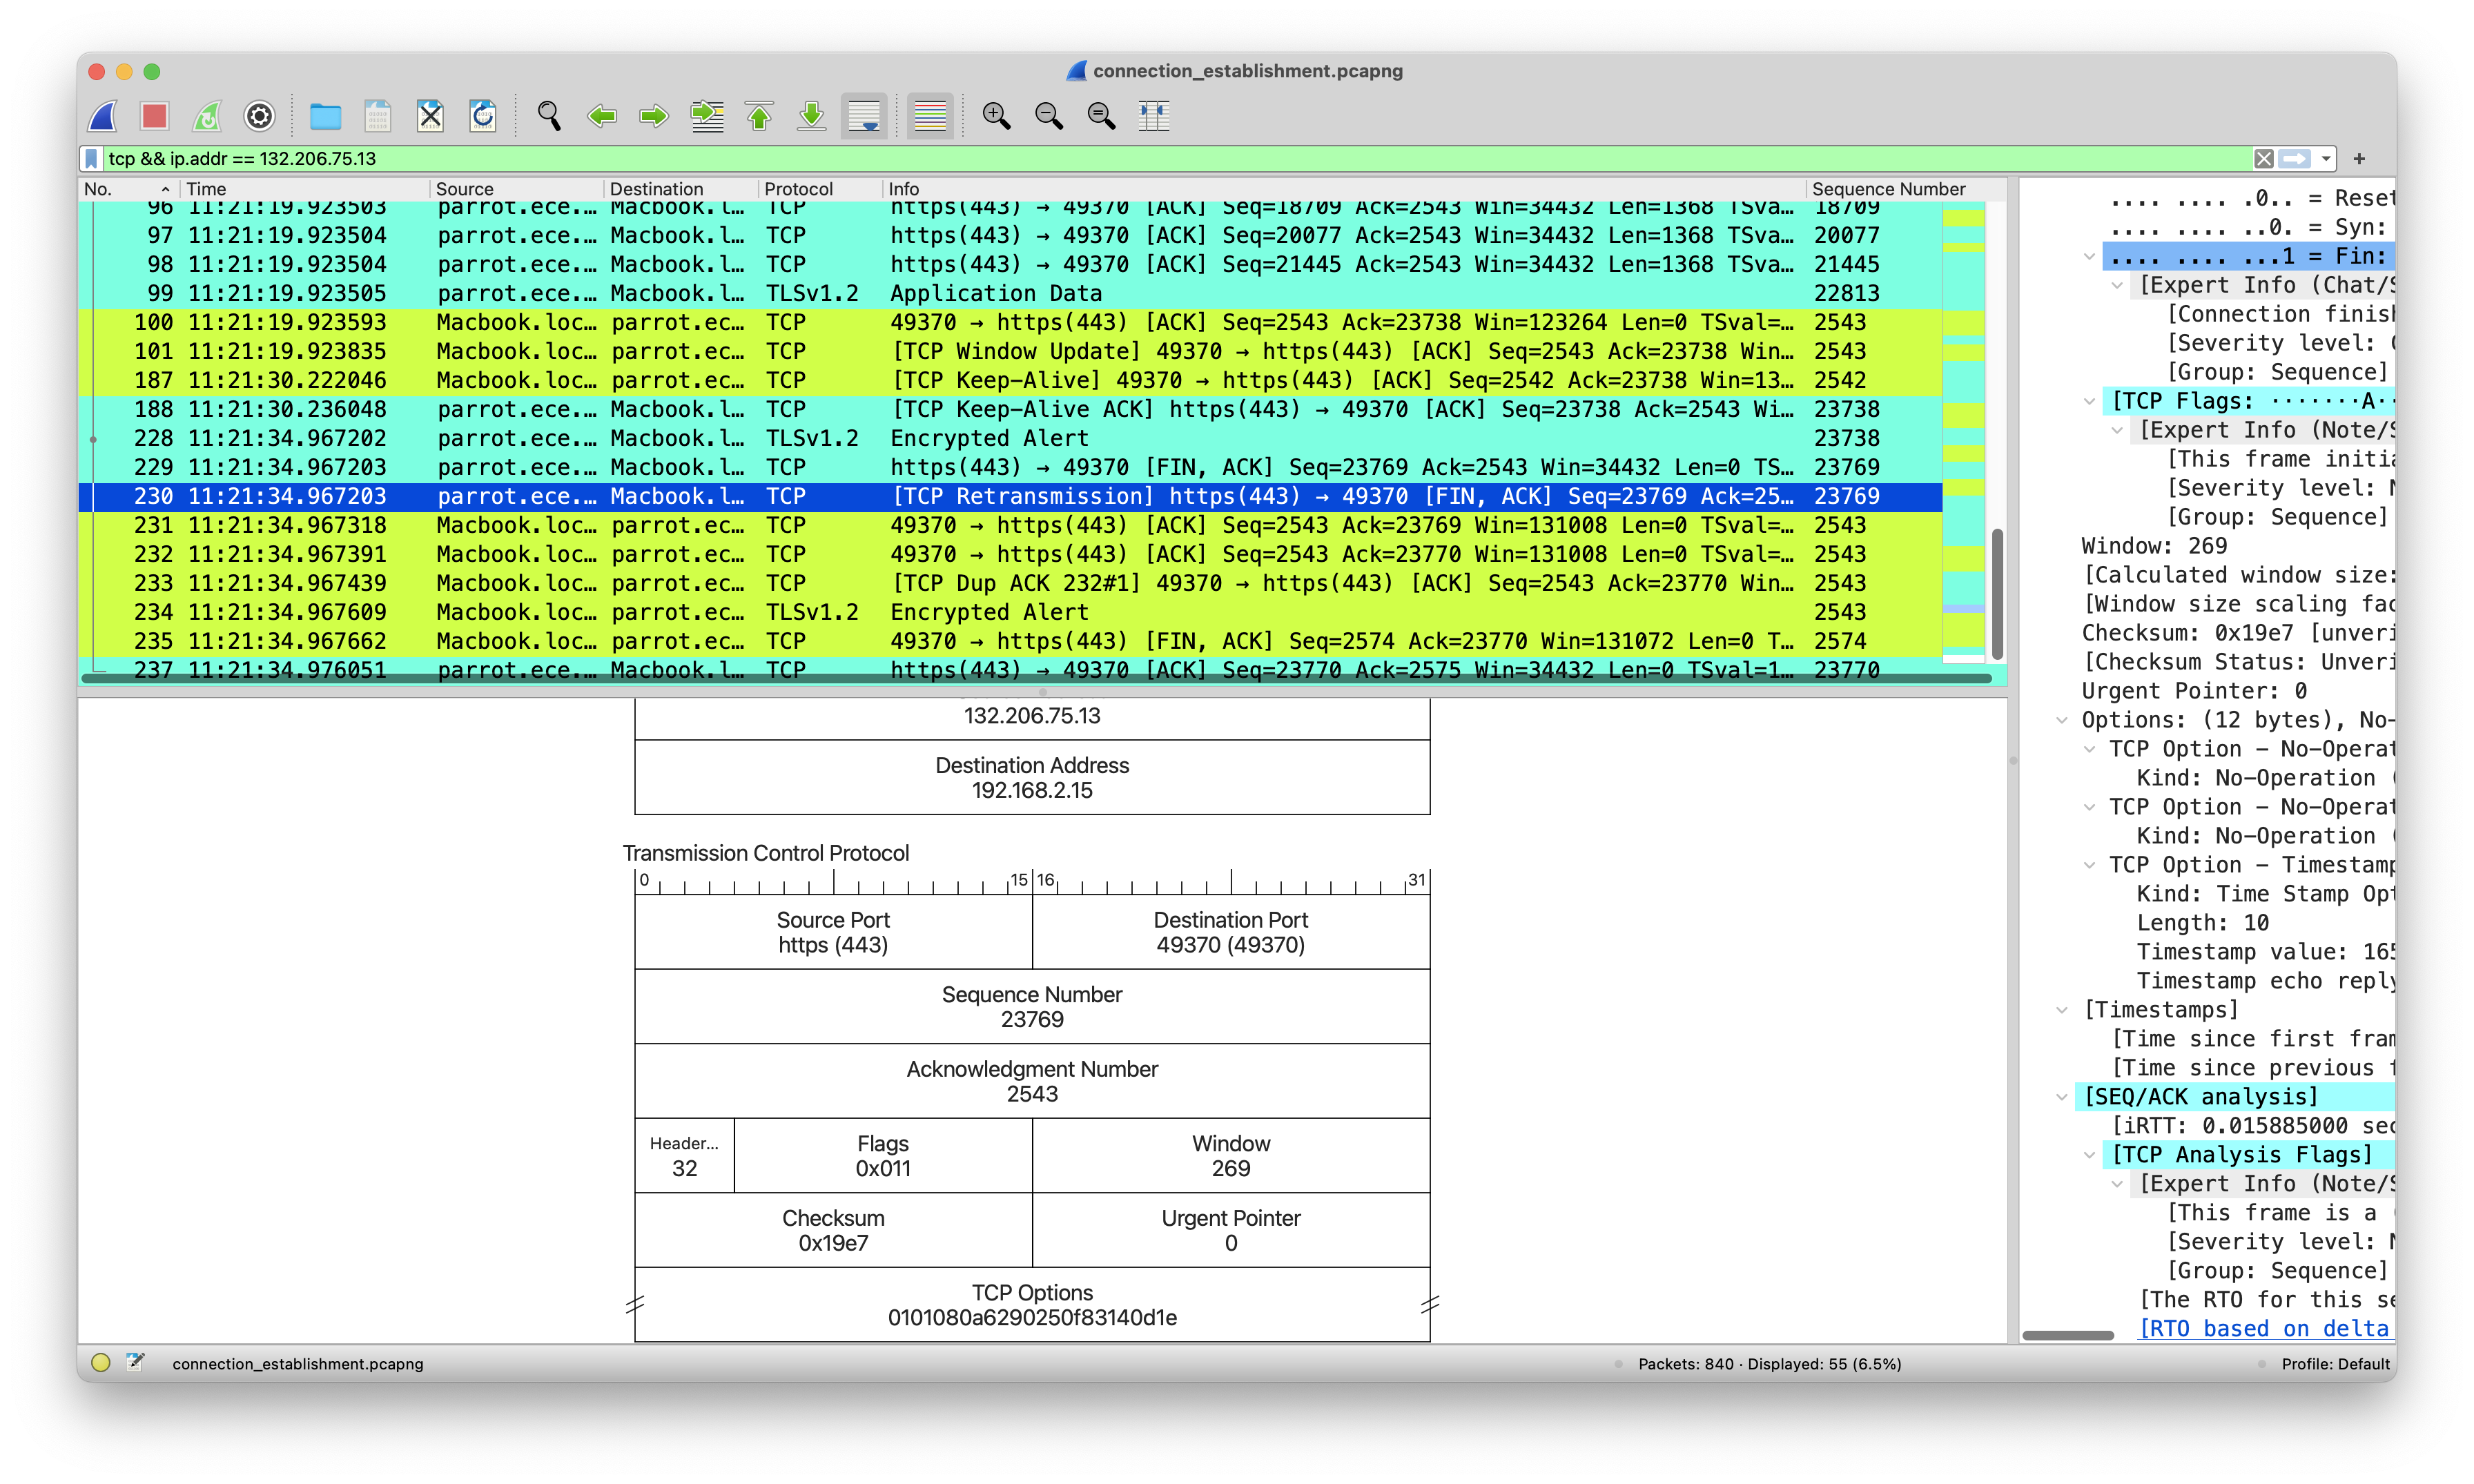
\includegraphics[width=\textwidth]{./images/RETRANSMISSION_SEGMENT_230_Q13}
\end{proof}
\newpage


\problem{14}
\begin{wts}
	How much data does the receiver typically acknowledge in an ACK? Can you identify cases where the receiver is ACKing every other received segment.
\end{wts}
\begin{proof}
% Answer here
    The amount of data varies, but the receiver ACKs every 5-6 segments. If the receiver were to ACK every segment, the this would be a waste of valuable network resources. Since TCP is a cumulative acknowledgement protocol. It suffices to ACK the last segment that was successfully received.\\

    Assuming the client (the author’s computer) is the receiver, it is clear from the two subsequent graphics that this is indeed the case, and the destination TCP ACKs every few kilobytes bytes.\\
	
    For more interactive applications such as telnet or SSH, we would expect the receiver to ACK every segment, as the the ACKs can piggyback off the TCP headers of the server-to-client segments. As opposed to the mostly uni-directional data transfer in our trace.
\end{proof}
\newpage


\problem{15}
\begin{wts}
	Calculate the throughput (bytes transferred per unit time) for the TCP connection? Explain how you obtained this value.
\end{wts}
\begin{proof}
% Answer here
    Consider the following graphics, which denote the throughput of the TCP connection.\\
    
    \textbf{Client to Server Throughput}\\
    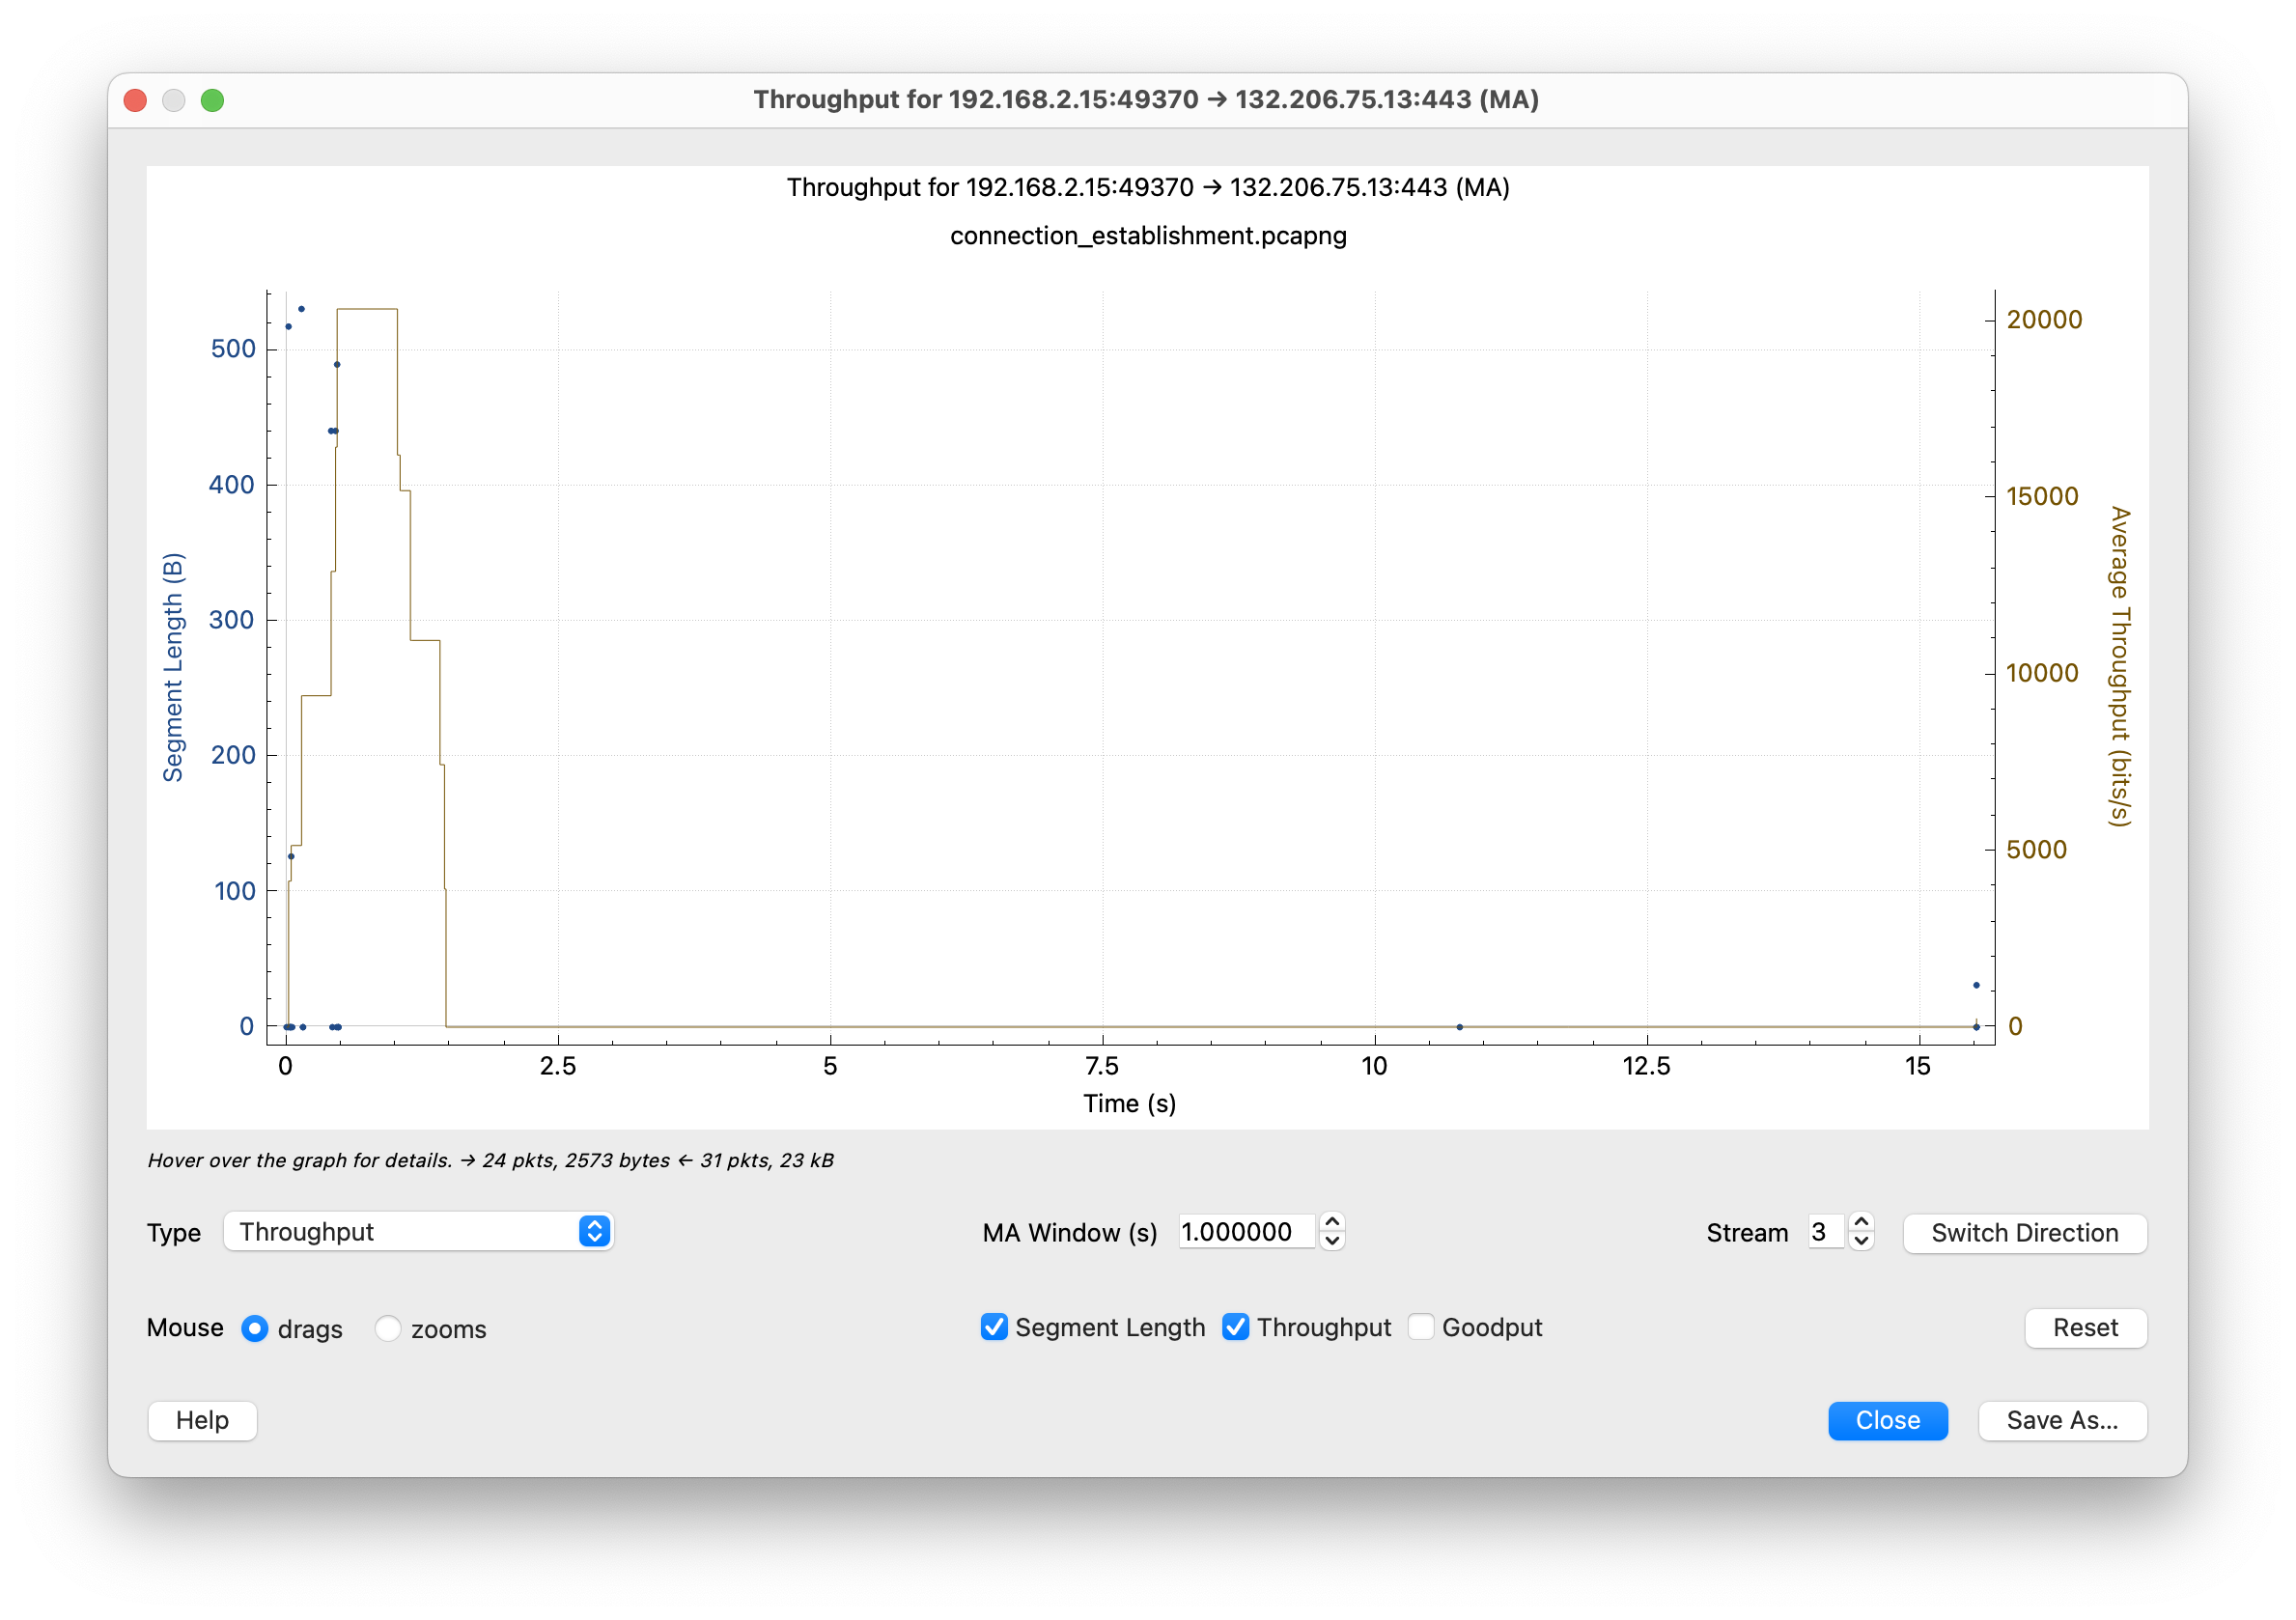
\includegraphics[width=\textwidth]{subfiles/images/throughput_Q15_client_to_server.png}
    
    \textbf{Server to Client Throughput}\\
    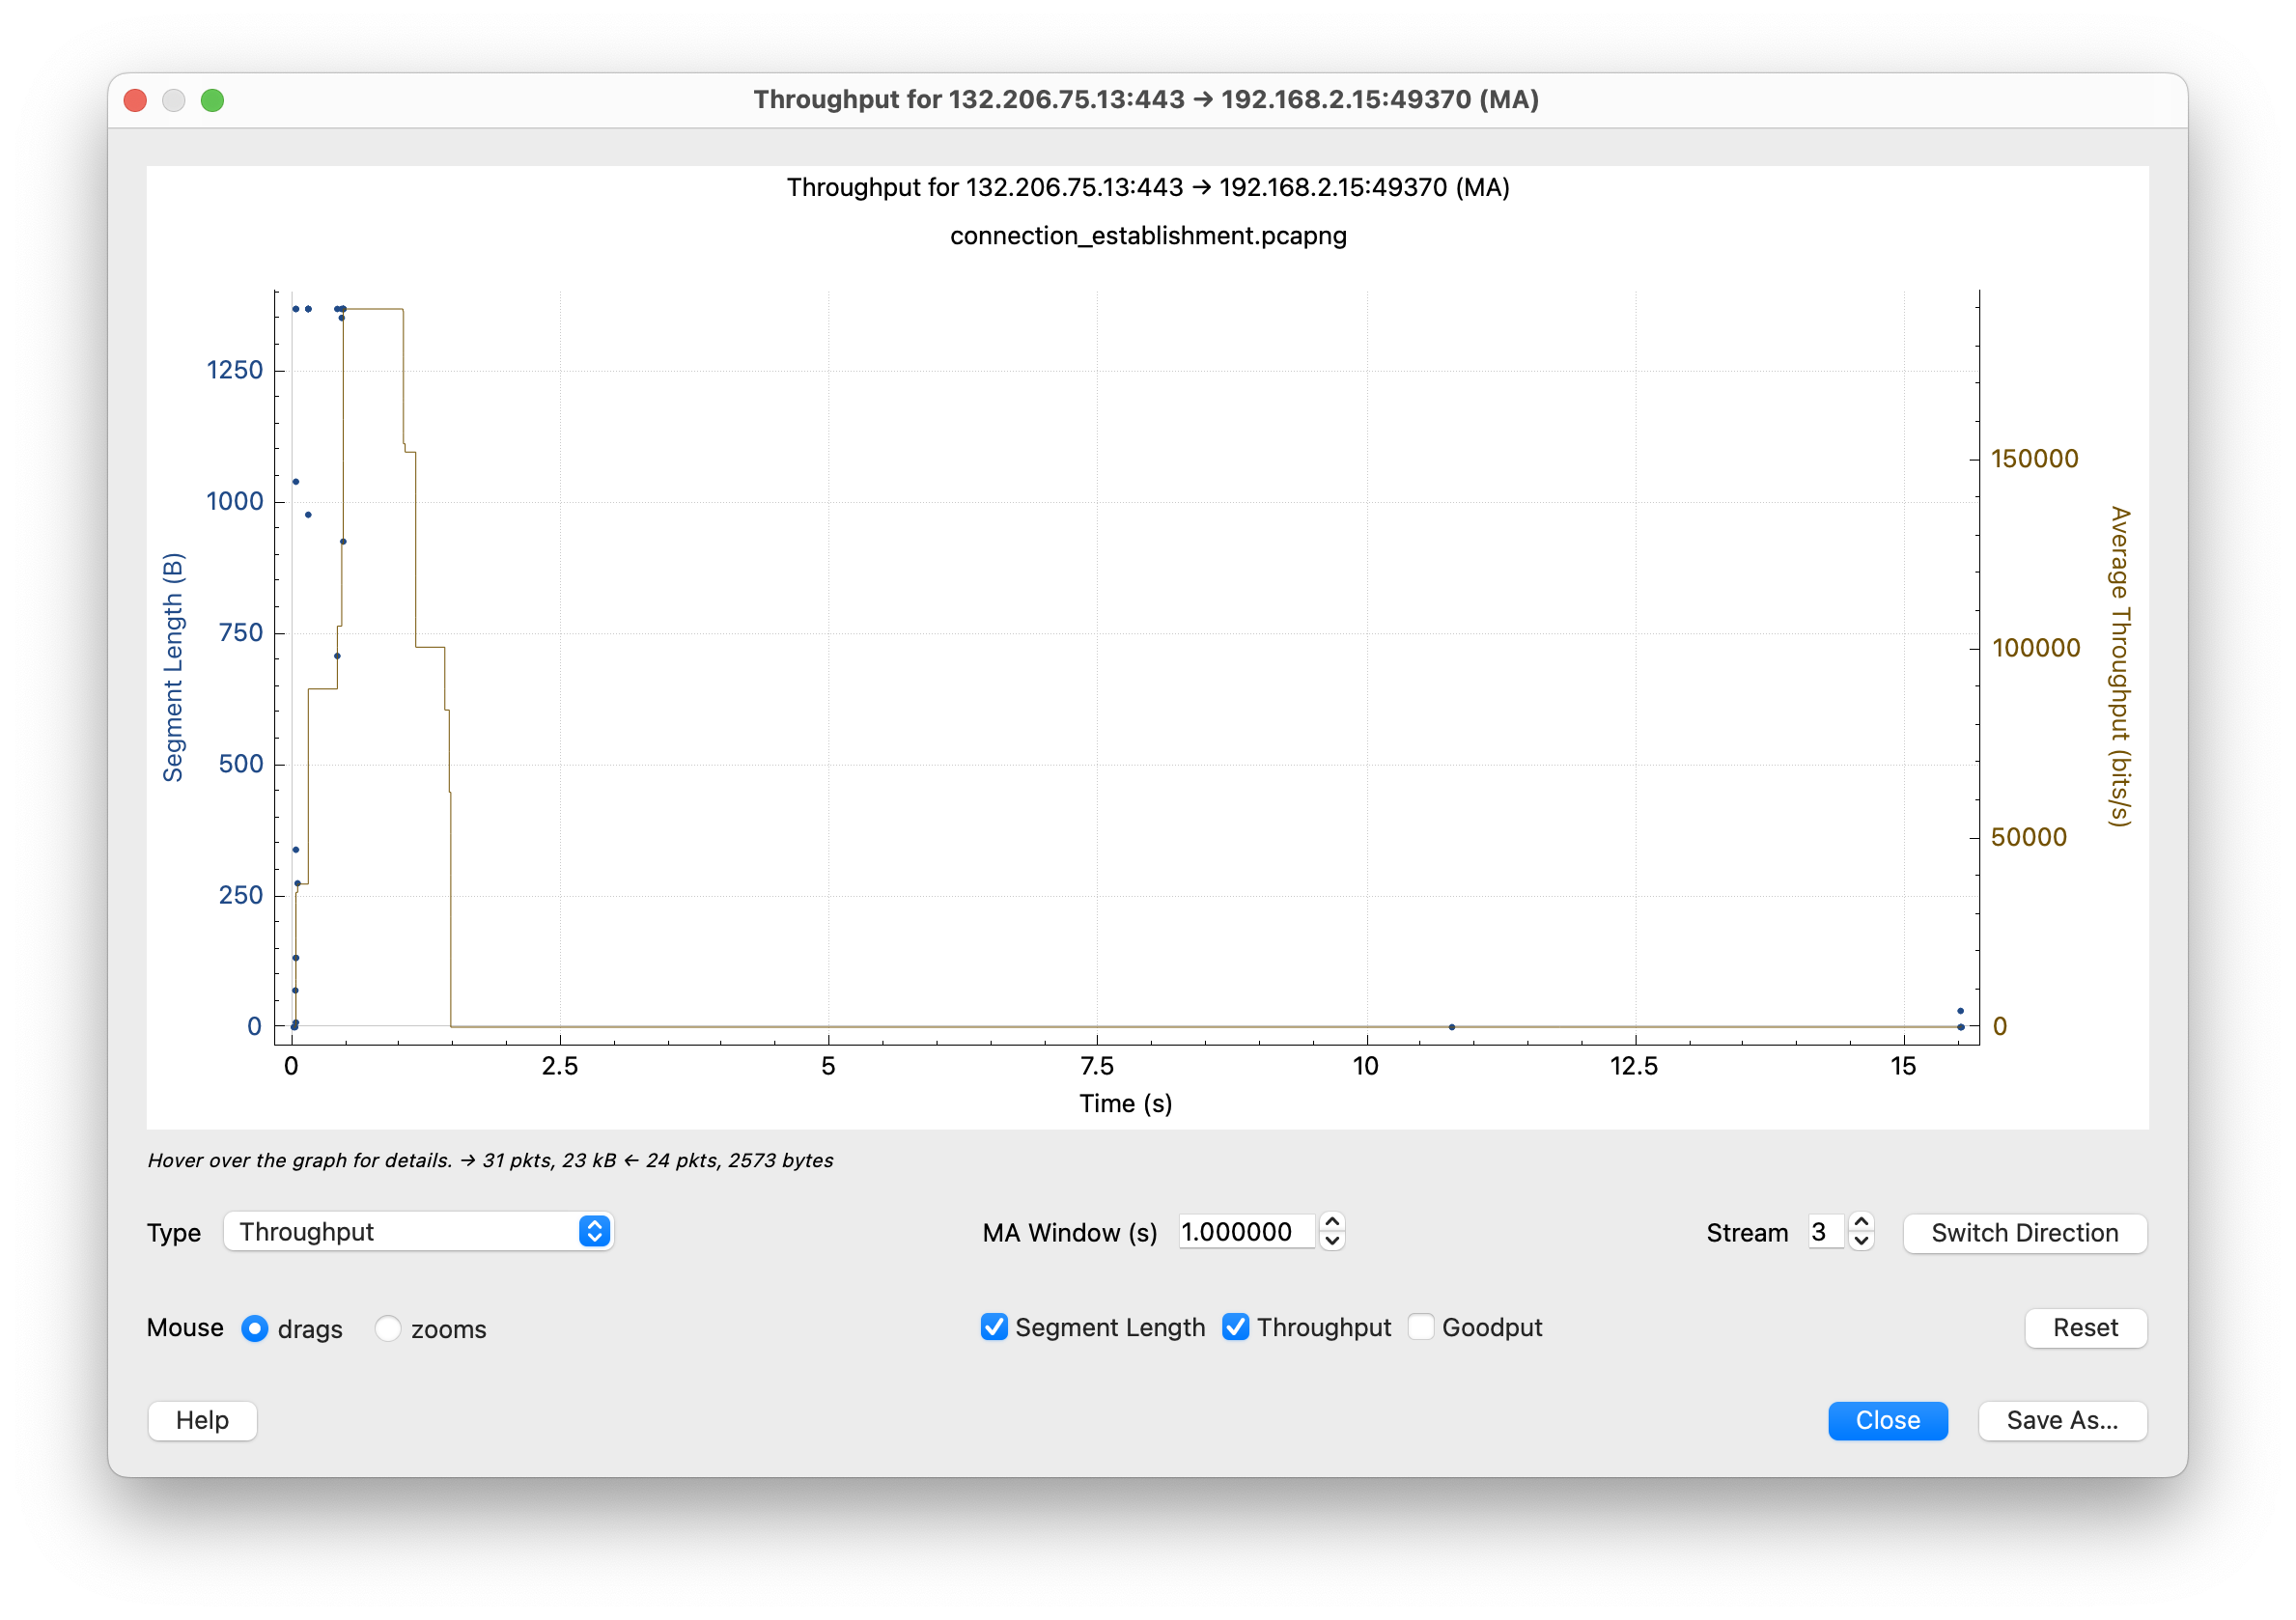
\includegraphics[width=\textwidth]{subfiles/images/throughput_Q15_server_to_client.png}
    
    The average throughput of the communication session is $500$Bps from the client to server. And $1350$Bps, in reverse, using the moving average.
\end{proof}
\newpage


\problem{16}
\begin{wts}
	How many TCP datagrams are exchanged for the termination phase?
\end{wts}
\begin{proof}
% Answer here
Four datagrams, this is clear from the following graphic.\\
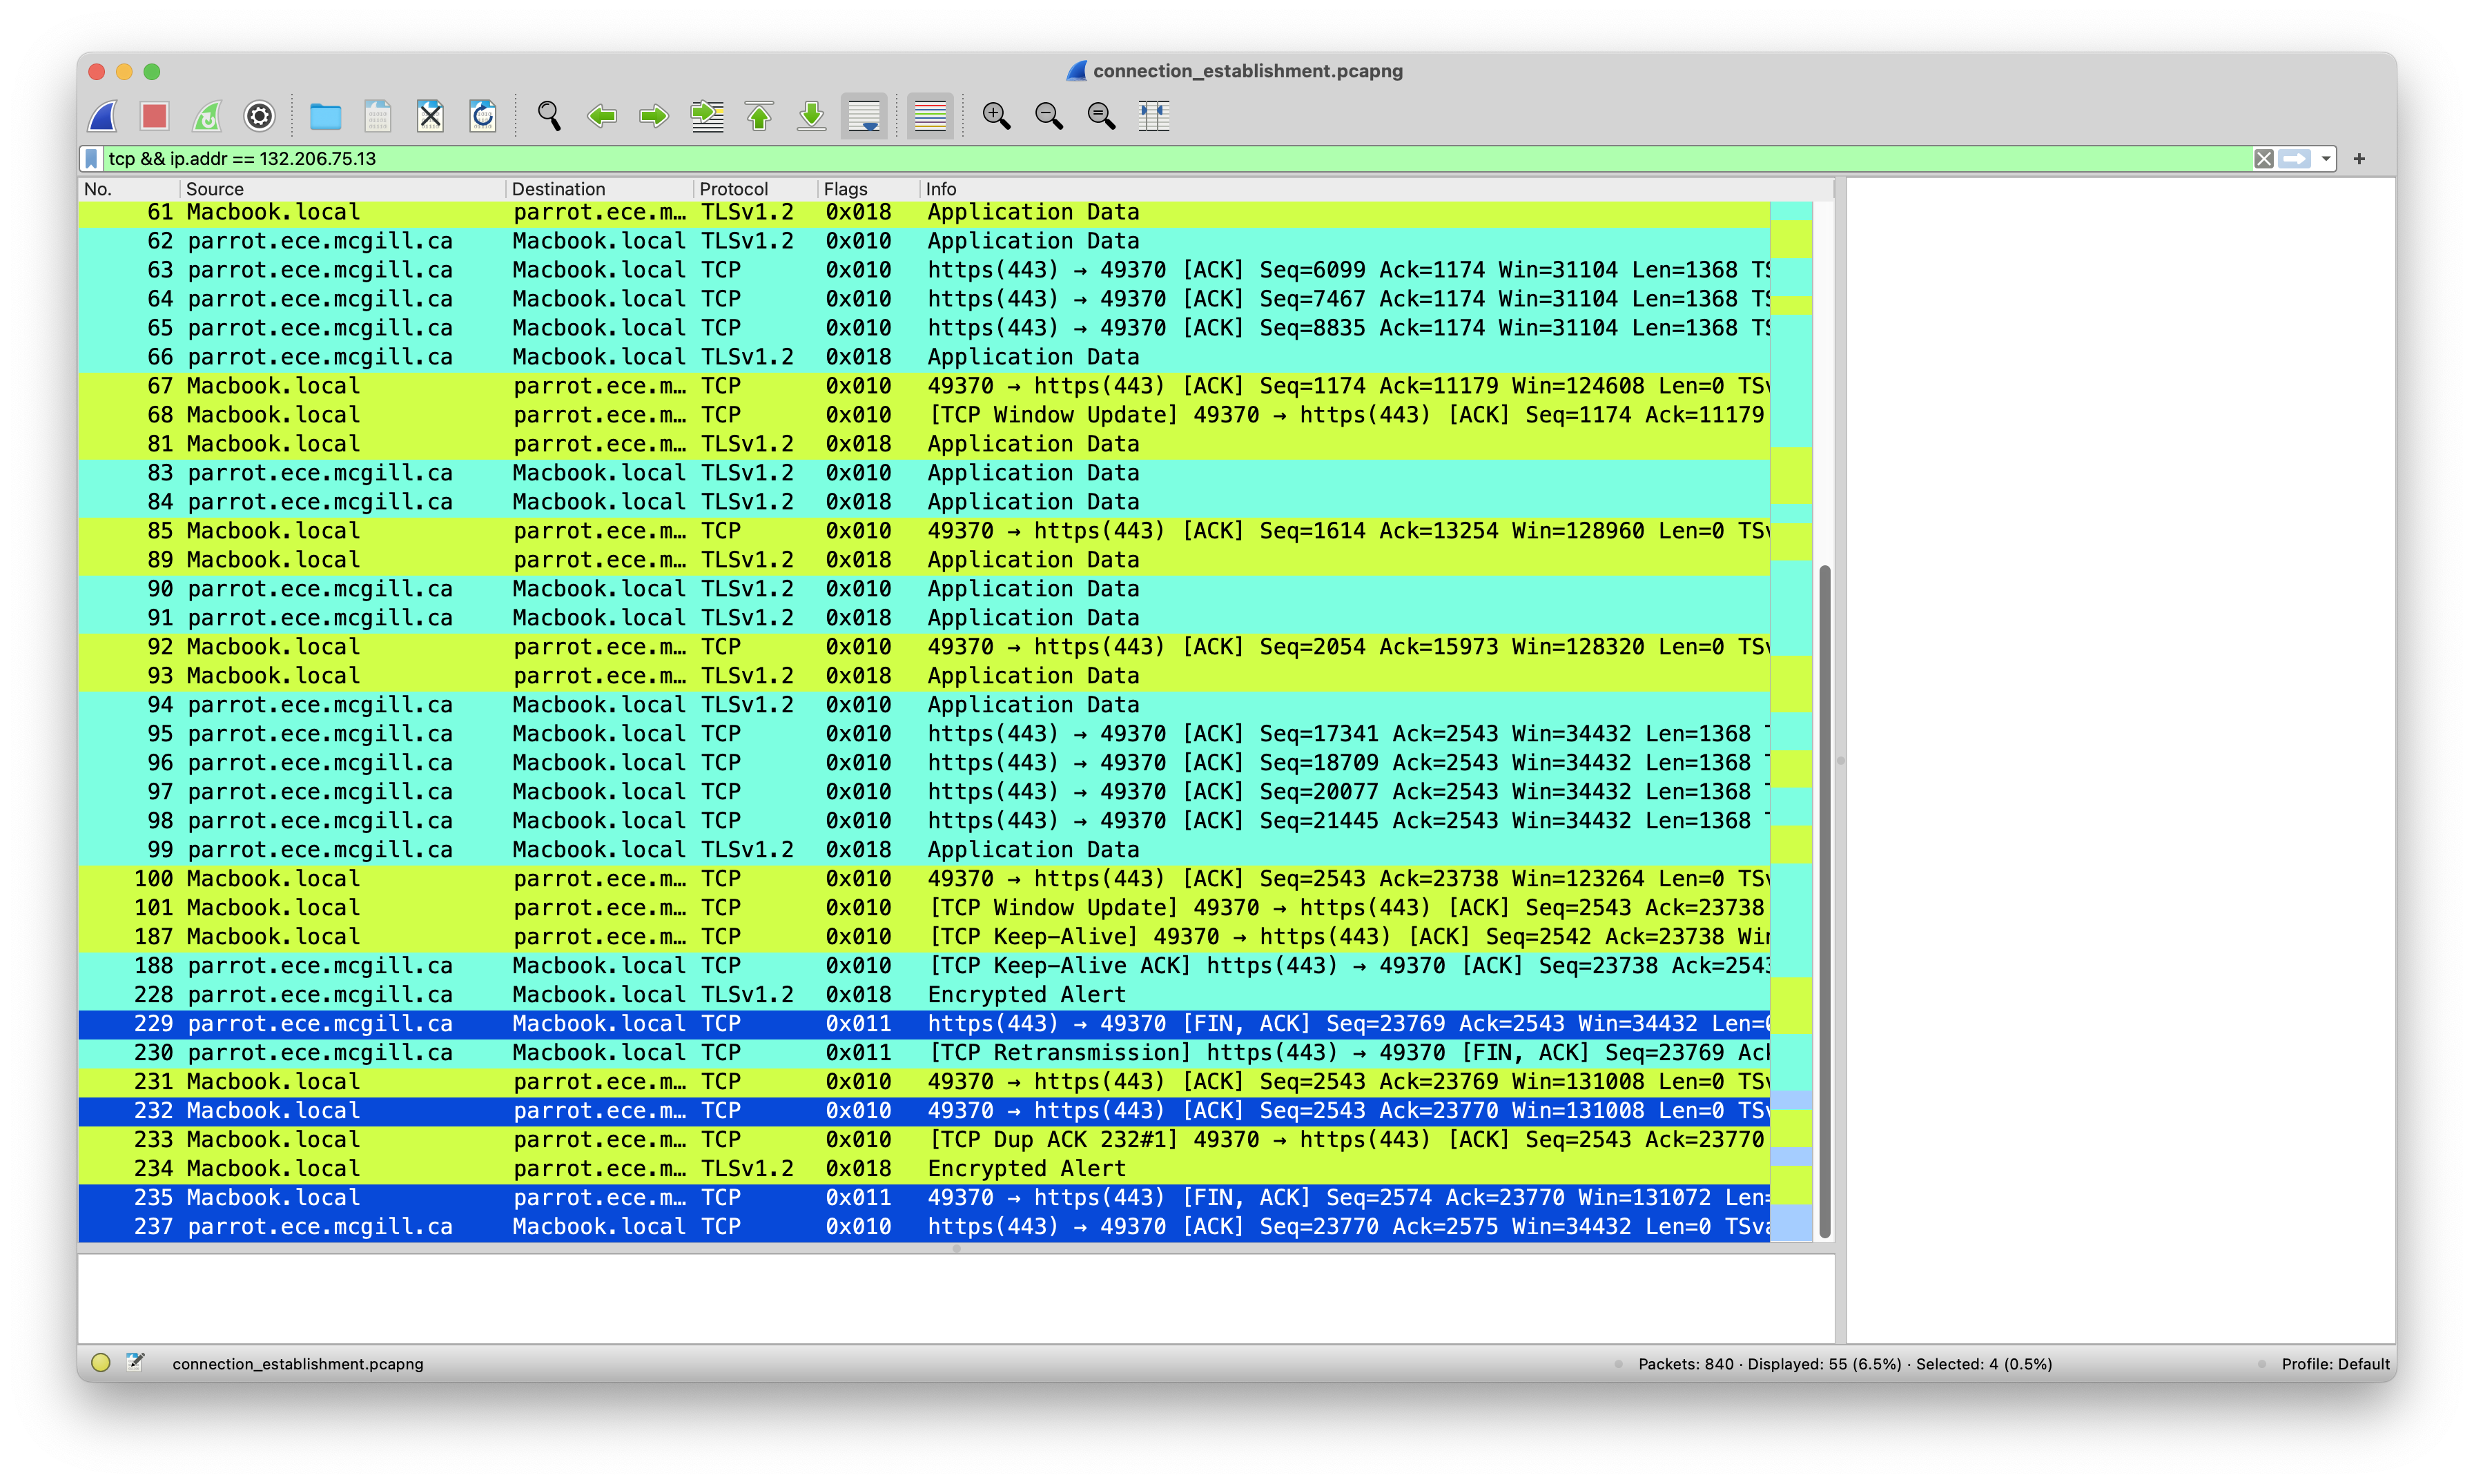
\includegraphics[width=\textwidth]{subfiles/images/CONNECTION_TERMINATION_Q16.png}
\textbf{Connection Termination Procedure}
\begin{enumerate}
    \item The server \code{parrot.ece.mcgill.ca} sends a TCP segment with \code{FIN = 1}, indicating that no more segments will be sent to the client
    \item The client acknowledges this segment with a separate ACK,
    \item Once the client finishes transmitting its messages, it sends a segment with \code{FIN = 1},
    \item The server acknowledges, and the connection is closed.
\end{enumerate}

\end{proof}
\newpage


\problem{17}
\begin{wts}
	Which end point started the Connection Termination phase?
\end{wts}
\begin{proof}
% Answer here
    The server initiates the connection teardown. See Problem 18.
\end{proof}
\newpage

\problem{18}
\begin{wts}
	What flags are set in each of segments used for connection termination?
\end{wts}
\begin{proof}
% Answer here
Consider the TCP Segments No. 229, 232, 235, 237.
\begin{itemize}
    \item Segment 229: Server to Client, Flags: \code{FIN, ACK}
    \begin{lstlisting}
    90 9c 4a bd 5d b0 64 66 24 ed 4d b8 08 00 45 00
    00 34 4f fa 40 00 33 06 65 37 84 ce 4b 0d c0 a8
    02 0f 01 bb c0 da 37 72 00 1a 01 a3 b5 9e 80 11
    01 0d 19 fd 00 00 01 01 08 0a 62 90 24 f9 83 14
    0d 1e\end{lstlisting}
    
    \item Segment 232: Client to Server, Flags: \code{ACK}
    \begin{lstlisting}
    64 66 24 ed 4d b8 90 9c 4a bd 5d b0 08 00 45 00
    00 34 00 00 40 00 40 06 a8 31 c0 a8 02 0f 84 ce
    4b 0d c0 da 01 bb 01 a3 b5 9e 37 72 00 1b 80 10
    07 ff d8 46 00 00 01 01 08 0a 83 14 47 e2 62 90
    24 f9\end{lstlisting}
    
    \item Segment 235: Client to Server, Flags: \code{FIN, ACK}
    \begin{lstlisting}
    64 66 24 ed 4d b8 90 9c 4a bd 5d b0 08 00 45 00
    00 34 00 00 40 00 40 06 a8 31 c0 a8 02 0f 84 ce
    4b 0d c0 da 01 bb 01 a3 b5 bd 37 72 00 1b 80 11
    08 00 d8 25 00 00 01 01 08 0a 83 14 47 e2 62 90
    24 f9\end{lstlisting}
    
    \item Segment 237: Server to Client, Flags: \code{ACK}
    \begin{lstlisting}
    90 9c 4a bd 5d b0 64 66 24 ed 4d bf 08 00 45 00
    00 34 4f fc 40 00 33 06 65 35 84 ce 4b 0d c0 a8
    02 0f 01 bb c0 da 37 72 00 1b 01 a3 b5 be 80 10
    01 0d de f0 00 00 01 01 08 0a 62 90 25 21 83 14
    47 e2\end{lstlisting}
\end{itemize}
\end{proof}
\newpage

\problem{19}
\begin{wts}
    Use the Time-Sequence-Graph (Stevens) plotting tool to view the sequence number versus time plot of segments being sent from the client to the server. Can you identify where TCP’s slow start phase begins and ends, and where congestion avoidance takes over? Explain your answer.
\end{wts}
\begin{proof}
    Consider the following graphic,\\
    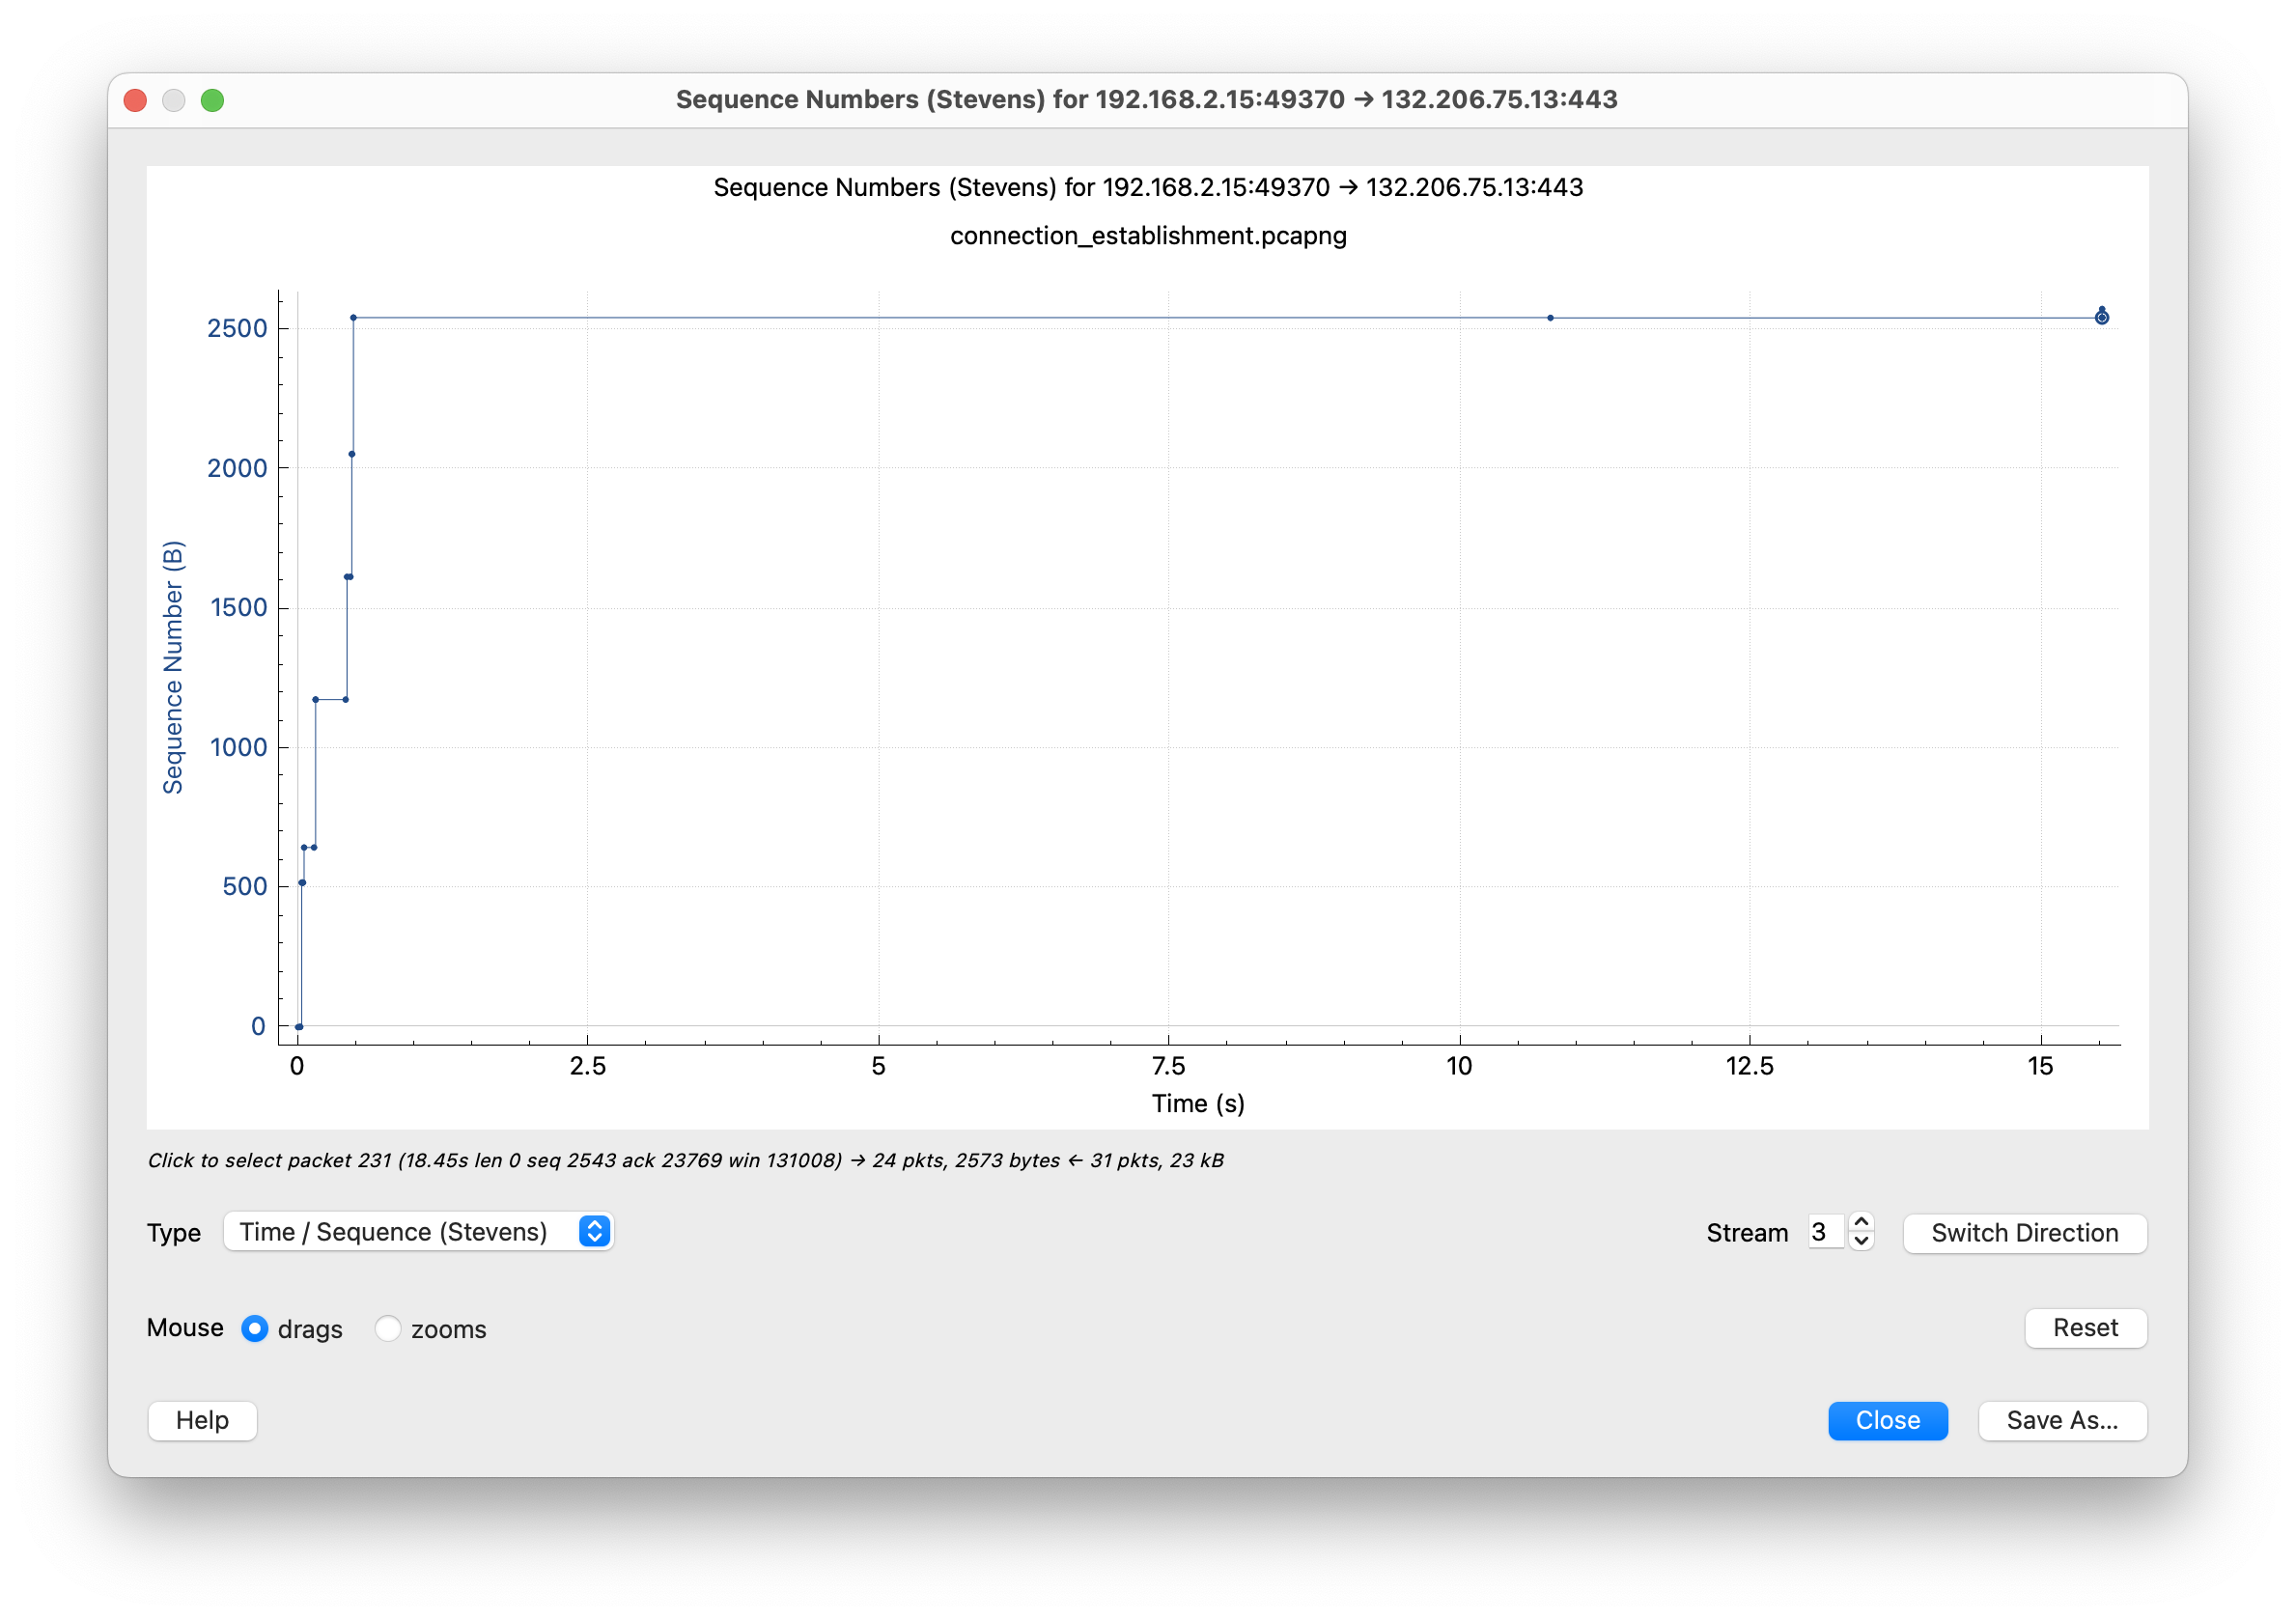
\includegraphics[width=\textwidth]{subfiles/images/connection_bytestream_plot_Q19_client_to_server.png}
    If we focus our attention towards the segments of significant lengths, then obviously the congestion avoidance phase never takes over. Since the increase in the sequence numbers do not decrease. However, this is but a pathological case in Reliable Data Transfer, as the number of bytes that are exchanged between the client and server are small. (The webpage is quite light-weight).\\
    
    Since no packets are dropped, the congestion window does not experience a significant decrease.
\end{proof}
\newpage

\problem{20}
\begin{wts}
    Locate the different phases of the congestion control mechanism on the below graph. Also describe the congestion control algorithm.\\
    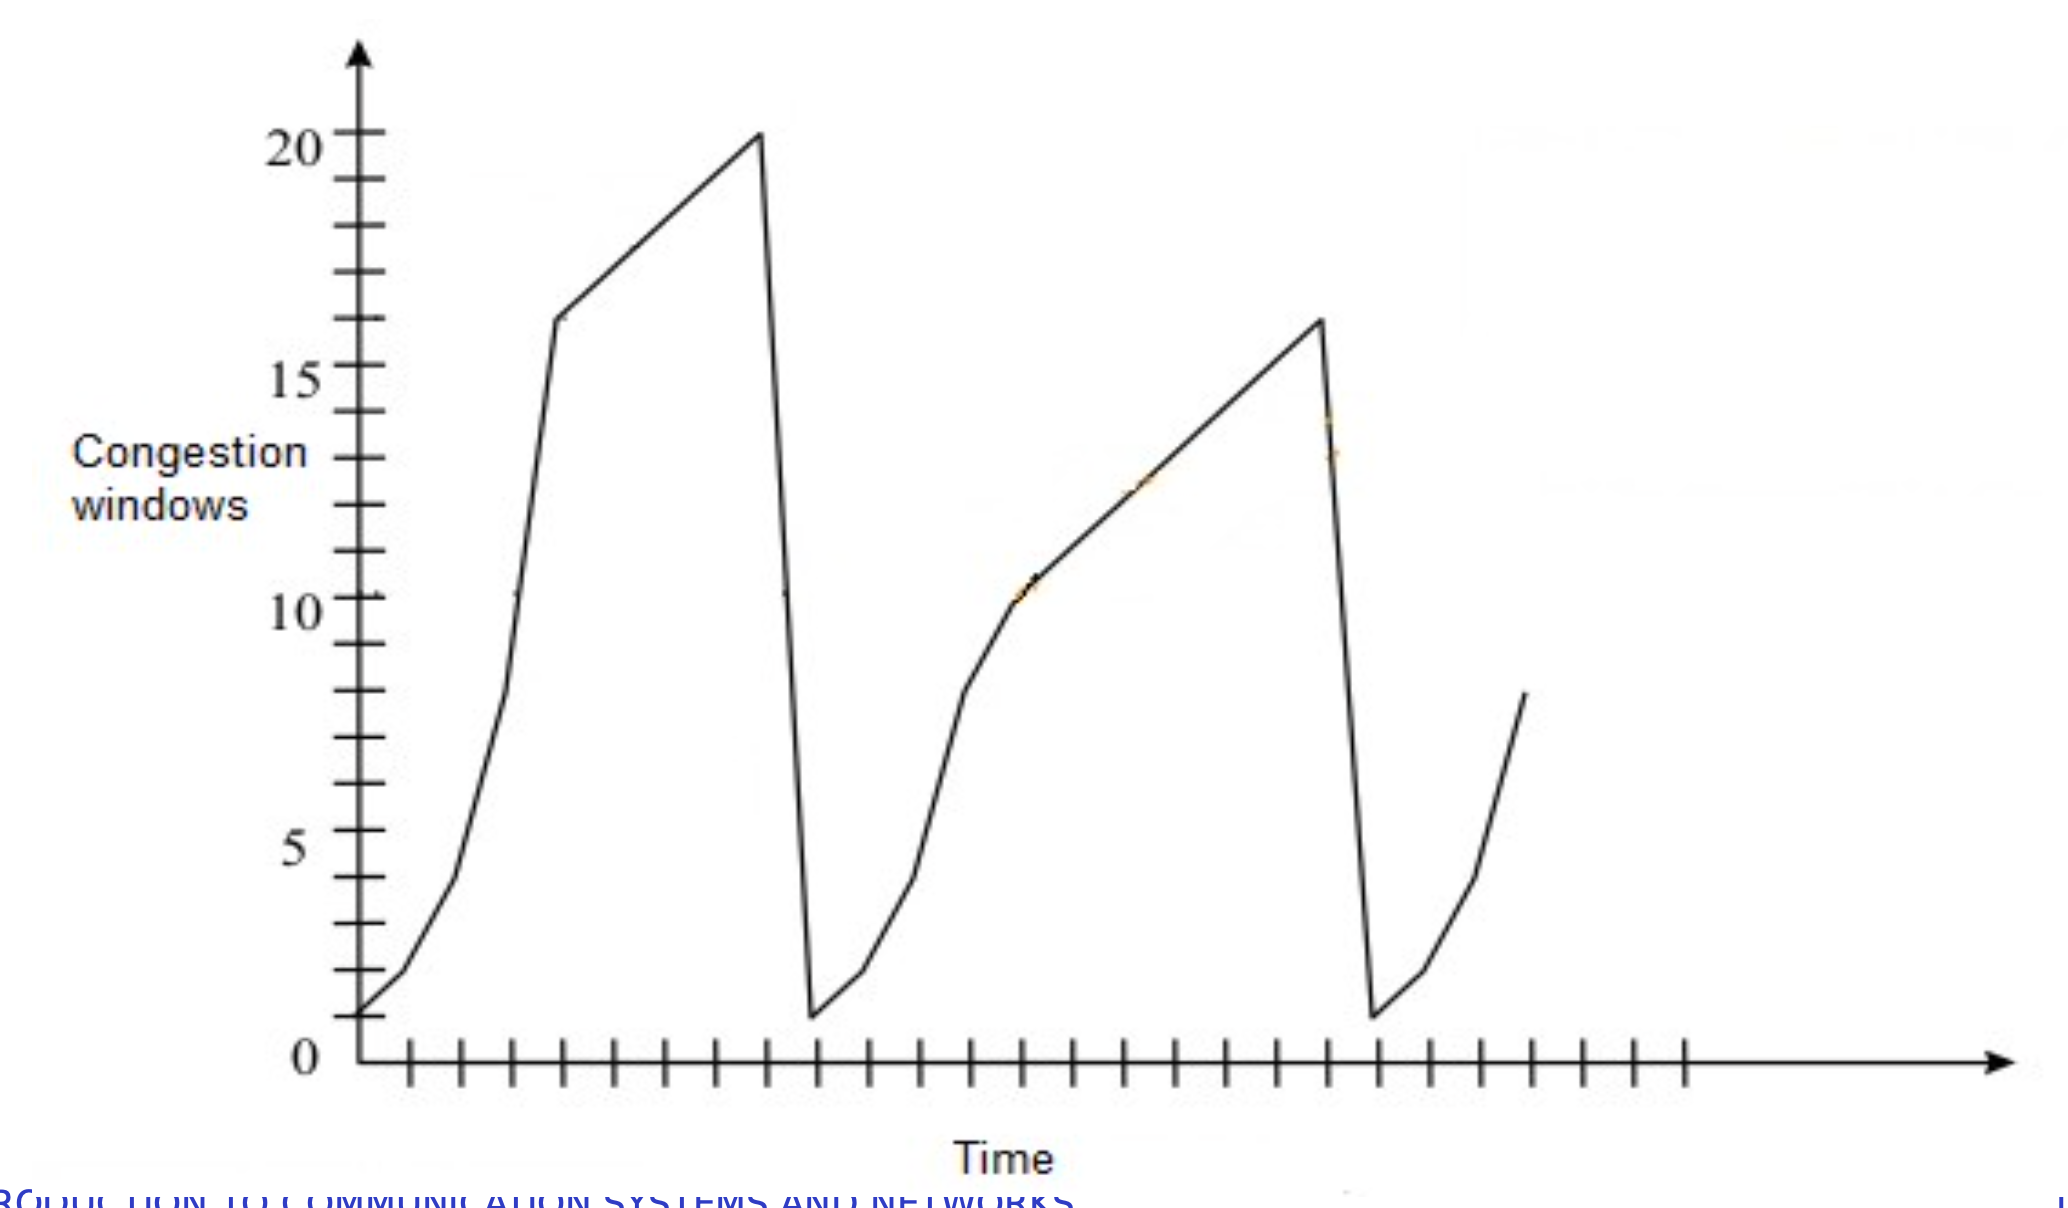
\includegraphics[width=\textwidth]{subfiles/images/part3_q19_window_graphic.png}
\end{wts}
\begin{proof}
The figure does not contain enough information to make a definitive conclusion. First, we do not know the units for time, whether they are in RTT, ERTT, SRTT, etc. Second, during the periods where the y-axis falls drastically to 1 dimensionless units, we do not know if it is caused by a true timeout or k-duplicate ACKs. Third, the units for the y-axis are missing. Does the MSS change with time during this protocol? This we can never know. To this, we will make three assumptions, one of which will have two cases. And in each of those two cases will yield — unsurprisingly, two different answers.
\begin{itemize}
    \item The axes are unitised with MSS and RTT respectively,
    \item The figure describes a protocol past its Connection Establishment phase,
    \item Either all of the y-drops are caused by timeouts, or none of them are. (And therefore caused by duplicate ACKs).
\end{itemize}

It is only after unveiling the ambiguity in the question, that anyone with his or her eyes open would be able to tell that the figure employs TCP Reno or Tahoe (exclusively at once), and TCP Tahoe. The discussion that follows assumes that all units of time are given in the discrete multiples of RTT, whereby assuming a symmetric LTI channel, and cwnd in multiples of MSS.\\

In a word, the operation of TCP Reno is based on the ability for the transmitter to distinguish between packets which are lost due to a timeout, which occurs only if multiple packets were lost during RTT — and packets which are lost individually. In the first case, TCP Reno sets ${ss}_{thresh}$ = cwnd/2, and — by invoking our second assumption —, resets cwnd to 1. On the subsequent RTT, TCP Reno is configured to be in Slow Start (terminating after cwnd=${ss}_{thresh}$) upon the immediate retransmission of the oldest lost segment.\\

In the second case, TCP Reno sets ${ss}_{thresh}$ = cwnd/2, and slashes cwnd by half. After retransmitting the lost segment, TCP Reno resumes using AIMD.\\

TCP Tahoe, does not distinguish between the two cases, and employs the second method of control, without regard whether the packets were lost in the atomic sense, or in unison.\\

Finally, both protocols are configured to start in Slow Start, with ${ss}_{thresh}$ ‘at infinity’ (in mathematical terms, taking ${ss}_{thresh}$ to be least of the ordinals that are greater — as directed by inclusion — than every initial segment of the first countable ordinals would suffice), and cwnd = 1.
\end{proof}
\end{document}
